% 第 21 章：递归类型的元理论
% Source: source/split/chapters/ch21-metatheory-of-recursive-types_p267-p300.pdf
% Original print pages: 281--314
% Status: 人工总审中

\chapter{递归类型的元理论}
\label{chap:21}

\section*{概览}

第 20 章介绍了递归类型的两种表示。等递归类型在定义上就等同于自身的展开；
同构递归类型则使用 \texttt{fold} 和 \texttt{unfold} 项，显式表示递归类型与其
展开之间的等价关系。本章为等递归类型的类型检查器建立理论基础；同构递归类型的
实现相对直接。实际语言经常把递归类型与子类型化结合起来，因此本章同时讨论
二者。即使去掉子类型化，系统也只会略微简单一些，因为类型检查器仍须判断两个
递归类型是否等价。

第 20 章曾用无限类型上的无限子类型推导，直观说明等递归类型的子类型关系。
本章将借助余归纳把这一理解精确化，并严格联系
无限树、无限推导与实际子类型算法所处理的有限表示。

\taplsecref{21.1}{sec:21.1}回顾归纳定义、余归纳定义及其证明原则；
\taplsecref{21.2}{sec:21.2}与\taplsecref{21.3}{sec:21.3}把一般理论用于
子类型关系，分别给出有限类型上的归纳定义和无限类型上的余归纳定义。
\taplsecref{21.4}{sec:21.4}短暂离开主线，讨论传递规则带来的一些问题
（正如前文所见，这条规则在子类型系统中一向是出了名的麻烦来源）；
\taplsecref{21.5}{sec:21.5}
给出检查归纳集合和余归纳集合成员关系的简单算法，\taplsecref{21.6}{sec:21.6}
进一步改进这些算法。\taplsecref{21.7}{sec:21.7}把算法用于正则无限类型；
\taplsecref{21.8}{sec:21.8}用有限的 \(\mu\)-类型表示无限类型，并证明
\(\mu\)-类型的子类型关系对应于无限类型上的普通余归纳定义。
\taplsecref{21.9}{sec:21.9}证明算法终止；\taplsecref{21.10}{sec:21.10}
把它与 Amadio 和 Cardelli 的算法比较；\taplsecref{21.11}{sec:21.11}简要讨论
同构递归类型的子类型化。\footnote{本章研究的系统，是带子类型化的简单类型演算
（\cref{fig:15-1}），再加上二元积（\cref{fig:11-5}）和等递归类型。原书配套
检查器名为 \texttt{equirec}。}

\section{归纳与余归纳}
\label{sec:21.1}

先固定一个全集 \(U\)，作为归纳定义和余归纳定义的论域。\(U\) 包含当前讨论中
所有可能的对象；归纳定义或余归纳定义的作用，是从中选出某个子集。稍后将取
\(U\) 为全部类型对的集合，使 \(U\) 的子集成为类型上的关系；眼下任意集合均可。

\begin{definition}
\label{def:21.1.1}
函数 \(F:\powerset(U)\to\powerset(U)\) 是\termfirst{单调的}{monotone}，若
\(X\subseteq Y\) 蕴含 \(F(X)\subseteq F(Y)\)。这里 \(\powerset(U)\) 表示
\(U\) 的所有子集组成的集合。
\end{definition}

本节以下假定 \(F\) 是 \(\powerset(U)\) 上的单调函数，并常称它为
\termfirst{生成函数}{generating function}。

\begin{definition}
\label{def:21.1.2}
设 \(X\subseteq U\)。
\begin{enumerate}
  \item 若 \(F(X)\subseteq X\)，则称 \(X\) 为 \(F\)-闭的；
  \item 若 \(X\subseteq F(X)\)，则称 \(X\) 为 \(F\)-一致的；
  \item 若 \(F(X)=X\)，则称 \(X\) 为 \(F\) 的不动点。
\end{enumerate}
\end{definition}

可以把 \(U\) 的元素看作陈述，把 \(F\) 看作一种“论证关系”：给定一组作为
前提的陈述，\(F\) 告诉我们能够推出哪些结论。一个 \(F\)-闭集合已经包含其成员
所能推出的全部结论；一个 \(F\)-一致集合中的每条陈述，都能由集合内的其他陈述
提供根据。\(F\) 的不动点同时满足这两个条件：成员需要的根据和成员能够推出的
结论都在集合中，除此以外没有别的元素。

\begin{example}
\label{exm:21.1.3}
在三元素全集 \(U=\{a,b,c\}\) 上考虑生成函数 \(E_1\)：
\[
\begin{array}{c@{\quad=\quad}c@{\qquad}c@{\quad=\quad}c}
E_1(\varnothing)&\{c\}&E_1(\{a,b\})&\{c\}\\
E_1(\{a\})&\{c\}&E_1(\{a,c\})&\{b,c\}\\
E_1(\{b\})&\{c\}&E_1(\{b,c\})&\{a,b,c\}\\
E_1(\{c\})&\{b,c\}&E_1(\{a,b,c\})&\{a,b,c\}
\end{array}
\]
唯一的 \(E_1\)-闭集合是 \(\{a,b,c\}\)；四个 \(E_1\)-一致集合是
\(\varnothing\)、\(\{c\}\)、\(\{b,c\}\) 和 \(\{a,b,c\}\)。

也可以用以下推导规则紧凑地表示 \(E_1\)：
\[
\frac{}{c}
\qquad
\frac{c}{b}
\qquad
\frac{b\quad c}{a}
\]
每条规则的含义是：若横线上方的元素都属于输入集合，横线下方的元素就属于
输出集合。
\end{example}

\taplstatementliststart
\begin{theorem}[Knaster--Tarski（Tarski，1955）]
\label{thm:21.1.4}
\taplstatementlistbreak
\begin{enumerate}
  \item 所有 \(F\)-闭集合的交，是 \(F\) 的最小不动点；
  \item 所有 \(F\)-一致集合的并，是 \(F\) 的最大不动点。
\end{enumerate}
\end{theorem}

\begin{proof}
只证第 2 项；第 1 项对称。令
\(\mathcal C=\{X\mid X\subseteq F(X)\}\)，即全部 \(F\)-一致集合组成的集合，
并令 \(P=\bigcup_{X\in\mathcal C}X\)。对任意 \(X\in\mathcal C\)，有
\[
X\subseteq F(X)\subseteq F(P),
\]
第二个包含关系来自 \(F\) 的单调性。对所有这样的 \(X\) 取并，得到
\(P\subseteq F(P)\)，所以 \(P\) 是 \(F\)-一致的；按定义，它也是最大的
\(F\)-一致集合。

再由单调性和 \(P\subseteq F(P)\)，得到
\(F(P)\subseteq F(F(P))\)，所以 \(F(P)\in\mathcal C\)。既然 \(P\) 是
\(\mathcal C\) 全部成员的并，便有 \(F(P)\subseteq P\)。合并两边的包含关系
可知 \(F(P)=P\)。因此 \(P\) 既是最大 \(F\)-一致集合，也是最大不动点。
\end{proof}

\begin{definition}
\label{def:21.1.5}
\(F\) 的最小不动点写作 \(\mu F\)，最大不动点写作 \(\nu F\)。
\end{definition}

\begin{example}
对\cref{exm:21.1.3}的生成函数 \(E_1\)，有
\(\mu E_1=\nu E_1=\{a,b,c\}\)。
\end{example}

\begin{exercise}[\(\star\)]
\label{ex:21.1.7}
设全集 \(\{a,b,c\}\) 上的生成函数 \(E_2\) 由以下规则定义：
\[
\frac{}{a}
\qquad
\frac{c}{b}
\qquad
\frac{a\quad b}{c}
\]
像\cref{exm:21.1.3}那样，显式列出关系 \(E_2\) 中的各个数对；列出所有
\(E_2\)-闭集合和 \(E_2\)-一致集合，并求 \(\mu E_2\) 与 \(\nu E_2\)。
\end{exercise}
\taplauthorsolutionlink{sol:author:21.1.7}{21.1.7}

注意，\(\mu F\) 本身是 \(F\)-闭的，因而是最小的 \(F\)-闭集合；\(\nu F\)
本身是 \(F\)-一致的，因而是最大的 \(F\)-一致集合。这给出两条基本推理原则。

\taplstatementliststart
\begin{corollary}
\label{cor:21.1.8}
\taplstatementlistbreak
\begin{enumerate}
  \item \textbf{归纳原理：}若 \(X\) 是 \(F\)-闭的，则 \(\mu F\subseteq X\)；
  \item \textbf{余归纳原理：}若 \(X\) 是 \(F\)-一致的，则 \(X\subseteq\nu F\)。
\end{enumerate}
\end{corollary}

把集合 \(X\) 看成谓词的特征集合，便容易理解这两条原则：证明性质 \(X\) 对
元素 \(x\) 成立，等价于证明 \(x\in X\)。归纳原理说，只要某个性质在 \(F\)
的作用下保持成立，也就是其特征集合对 \(F\) 闭合，那么它就对归纳定义集合
\(\mu F\) 的全部元素成立。

余归纳原理则给出证明 \(x\in\nu F\) 的办法：只需找到一个包含 \(x\) 的
\(F\)-一致集合 \(X\)。余归纳虽然不如归纳熟悉，却是许多计算机科学领域的
核心工具，例如并发理论中的\termfirst{互模拟}{bisimulation}和许多
\termfirst{模型检查}{model checking}算法。

\translatornote{互模拟用于比较两个状态转移系统。若某个关系中的一对状态满足：
一方的每一步转移都能由另一方匹配，并且转移后得到的两个状态仍处于这个关系中；
反方向也满足同样的条件，那么这个关系就是互模拟。所有互模拟关系的并仍是
互模拟，因此可以用最大不动点和余归纳来刻画。模型检查则是在状态转换图上自动
判断系统是否满足给定性质；其中许多算法同样可以表述为计算最小或最大不动点。}

本章会反复使用归纳与余归纳。为简洁起见，归纳论证常写作结构归纳等熟悉形式，
不再每次都展开为生成函数和谓词；余归纳论证则会写得更明确。

\begin{exercise}[推荐，\(\star\star\star\)]
\label{ex:21.1.9}
证明：自然数上的普通归纳原理（\cref{ax:2.4.1}）以及自然数对上的字典序归纳
原理（\cref{ax:2.4.4}），都可以从\cref{cor:21.1.8}的归纳原理推出。
\end{exercise}
\taplauthorsolutionlink{sol:author:21.1.9}{21.1.9}

\section{有限类型与无限类型}
\label{sec:21.2}

接下来要把最大不动点和余归纳证明法用于子类型关系。为此，先精确定义怎样把
类型视为有限树或无限树。本章只使用三种类型构造子：\(\to\)、\(\times\) 和
\(\tapltype{Top}\)。树的每个节点都用其中一个符号标记。下面的定义只针对本章
所需的树；无限带标签树的一般理论可参阅 Courcelle（1983）。

令 \(\{1,2\}^{*}\) 表示由 1 和 2 组成的全部有限序列，空序列记为
\(\epsilon\)，\(i^k\) 表示 \(k\) 个 \(i\) 连成的序列；若 \(\pi\) 和
\(\sigma\) 都是序列，则 \(\pi,\sigma\) 表示二者的连接。

\begin{definition}
\label{def:21.2.1}
\termfirst{树类型}{tree type}（简称树）是满足以下条件的偏函数\footnote{“树
类型”这个说法略显别扭，但有助于和\taplsecref{21.8}{sec:21.8}将要讨论的另一种
有限表示相区分；后者称为“\(\mu\)-类型”。}
\[
T:\{1,2\}^{*}\rightharpoonup\{\to,\times,\tapltype{Top}\}.
\]
\begin{enumerate}
  \item \(T(\epsilon)\) 有定义；
  \item 若 \(T(\pi,\sigma)\) 有定义，则 \(T(\pi)\) 有定义；
  \item 若 \(T(\pi)=\to\) 或 \(T(\pi)=\times\)，则
        \(T(\pi,1)\) 与 \(T(\pi,2)\) 都有定义；
  \item 若 \(T(\pi)=\tapltype{Top}\)，则
        \(T(\pi,1)\) 与 \(T(\pi,2)\) 都无定义。
\end{enumerate}
若 \(\dom(T)\) 有限，则称 \(T\) 为有限树类型。所有树类型的集合记作
\(\mathcal T\)，其中全部有限树类型组成的子集记作 \(\mathcal T_f\)。
\end{definition}

为方便记号，\(\tapltype{Top}\) 也表示唯一节点标为 \(\tapltype{Top}\) 的树。
若 \(T_1,T_2\) 是树，则 \(T_1\times T_2\) 和 \(T_1\to T_2\) 分别表示由
以下函数定义的树，其中 \(i=1,2\)：
\[
\begin{aligned}
(T_1\times T_2)(\epsilon)&=\times,
& (T_1\times T_2)(i,\pi)&=T_i(\pi),\\
(T_1\to T_2)(\epsilon)&=\to,
& (T_1\to T_2)(i,\pi)&=T_i(\pi)
\end{aligned}
\]
例如，
\((\tapltype{Top}\times\tapltype{Top})\to\tapltype{Top}\) 表示有限树
\[
T(\epsilon)=\to,\quad T(1)=\times,\quad
T(2)=T(1,1)=T(1,2)=\tapltype{Top}.
\]
省略号可用于非有限树。例如，
\(\tapltype{Top}\to(\tapltype{Top}\to(\tapltype{Top}\to\cdots))\)
对应的树满足：对每个 \(k\ge0\)，\(T(2^k)=\to\) 且
\(T(2^k,1)=\tapltype{Top}\)。

\begin{figure}[!ht]
\centering
\begin{tikzpicture}[
  level distance=11mm,
  level 1/.style={sibling distance=32mm},
  level 2/.style={sibling distance=22mm},
  every node/.style={font=\small}
]
\node at (-3.4,0) {$\to$}
  child {node {$\times$}
    child {node {$\tapltype{Top}$} edge from parent node[left] {\scriptsize 1}}
    child {node {$\tapltype{Top}$} edge from parent node[right] {\scriptsize 2}}
    edge from parent node[left] {\scriptsize 1}}
  child {node {$\tapltype{Top}$} edge from parent node[right] {\scriptsize 2}};
\node at (2.4,0) {$\to$}
  child {node {$\tapltype{Top}$} edge from parent node[left] {\scriptsize 1}}
  child {node {$\to$}
    child {node {$\tapltype{Top}$} edge from parent node[left] {\scriptsize 1}}
    child {node {$\vdots$} edge from parent node[right] {\scriptsize 2}}
    edge from parent node[right] {\scriptsize 2}};
\node[below=34mm] at (-3.4,0)
  {$({\tapltype{Top}}\times{\tapltype{Top}})\to\tapltype{Top}$};
\node[below=34mm] at (2.4,0)
  {$\tapltype{Top}\to(\tapltype{Top}\to\cdots)$};
\end{tikzpicture}
\caption{树类型示例}
\label{fig:21-1}
\end{figure}

有限树类型还可以用文法紧凑定义：
\[
T ::= \tapltype{Top}\mid T\times T\mid T\to T.
\]
形式上，\(\mathcal T_f\) 是该文法所描述生成函数的最小不动点。该生成函数以
所有由 \(\tapltype{Top}\)、\(\to\) 和 \(\times\) 标记的有限树和无限树为全集；
换言之，在\cref{def:21.2.1}中删去最后两项条件，就得到这个全集。同一生成函数
取最大不动点，便得到全部树类型 \(\mathcal T\)。

\translatornote{把上述文法理解成作用于树集合的函数，可以看清它与不动点的
关系。对任意树集合 \(X\)，定义
\[
F(X)=\{\tapltype{Top}\}
\cup\{T_1\times T_2\mid T_1,T_2\in X\}
\cup\{T_1\to T_2\mid T_1,T_2\in X\}
\]
也就是说，\(F\) 总能生成单节点树 \(\tapltype{Top}\)，还可以用 \(X\) 中的
两棵树作为左右子树，生成一棵新的积类型树或箭头类型树。

从空集开始反复应用 \(F\)，第一个阶段得到 \(\tapltype{Top}\)，以后每个阶段
都在已有树的外面增加一层。任意一个阶段只含深度有界的有限树；把所有阶段的
结果取并，便得到 \(\mathcal T_f\)。\(\mathcal T_f\) 本身是无穷集合，但其中
每一棵树都是有限的。用两棵有限树再构造一层，结果仍是有限树；反过来，任意
有限树或者就是 \(\tapltype{Top}\)，或者可以在根节点处拆成两棵有限子树。
因此 \(F(\mathcal T_f)=\mathcal T_f\)，所以 \(\mathcal T_f\) 是 \(F\) 的一个
不动点。它还是最小的不动点：任取另一个不动点 \(Y\)，由 \(F(Y)=Y\) 可知
\(Y\) 必须包含 \(\tapltype{Top}\)，并且只要包含 \(T_1,T_2\)，就必须同时
包含 \(T_1\times T_2\) 和 \(T_1\to T_2\)。按照有限树的构造逐层应用这条
性质，可以得到 \(\mathcal T_f\subseteq Y\)。因此，每个不动点都至少包含
全部有限树，不可能比 \(\mathcal T_f\) 更小。

同一生成函数的最大不动点还会收入无限向下展开的树。这类树不会在上述任何
有限阶段出现，但它的根节点和两棵直接子树仍然满足相同的生成条件。因此，
\(\mu F=\mathcal T_f\) 给出全部有限树类型，\(\nu F=\mathcal T\) 则给出全部
有限或无限树类型。}

\begin{exercise}[推荐，\(\star\star\)]
\label{ex:21.2.2}
沿用上一段的思路，给出全集 \(U\) 和生成函数
\(F:\powerset(U)\to\powerset(U)\)，使有限树类型集合 \(\mathcal T_f\)
等于 \(\mu F\)，全部树类型集合 \(\mathcal T\) 等于 \(\nu F\)。
\end{exercise}
\taplauthorsolutionlink{sol:author:21.2.2}{21.2.2}

\section{子类型化}
\label{sec:21.3}

有限树类型上的子类型关系和任意树类型上的子类型关系，将分别定义为某个单调
函数的最小不动点和最大不动点。有限情形的全集是
\(\mathcal T_f\times\mathcal T_f\)。这个全集的子集就是有限树类型上的关系；
生成函数把这样的关系映射到同一全集中的另一个关系，所以该生成函数的各个
不动点也都是有限树类型上的关系。无限情形的全集则是
\(\mathcal T\times\mathcal T\)。

\begin{definition}[有限子类型关系]
\label{def:21.3.1}
若 \((S,T)\in\mu\mathcal S_f\)，则称有限树类型 \(S\) 是 \(T\) 的子类型。
单调函数
\(\mathcal S_f:\powerset(\mathcal T_f\times\mathcal T_f)
\to\powerset(\mathcal T_f\times\mathcal T_f)\) 定义为
\[
\begin{aligned}
\mathcal S_f(R)={}&\{(T,\tapltype{Top})\mid T\in\mathcal T_f\}\\
&\cup\{(S_1\times S_2,T_1\times T_2)
          \mid (S_1,T_1),(S_2,T_2)\in R\}\\
&\cup\{(S_1\to S_2,T_1\to T_2)
          \mid (T_1,S_1),(S_2,T_2)\in R\}.
\end{aligned}
\]
\end{definition}

该函数与熟悉的三条子类型规则完全对应：
\[
\frac{}{T\subtype\tapltype{Top}}
\qquad
\frac{S_1\subtype T_1\quad S_2\subtype T_2}
     {S_1\times S_2\subtype T_1\times T_2}
\qquad
\frac{T_1\subtype S_1\quad S_2\subtype T_2}
     {S_1\to S_2\subtype T_1\to T_2}.
\]
横线上方的 \(S\subtype T\) 表示“类型对 \((S,T)\) 属于
\(\mathcal S_f\) 的输入关系”，横线下方则表示该类型对属于输出关系。

\begin{definition}[无限子类型关系]
\label{def:21.3.2}
若 \((S,T)\in\nu\mathcal S\)，则称树类型 \(S\) 是 \(T\) 的子类型，其中
\(\mathcal S:\powerset(\mathcal T\times\mathcal T)
\to\powerset(\mathcal T\times\mathcal T)\) 定义为
\[
\begin{aligned}
\mathcal S(R)={}&\{(T,\tapltype{Top})\mid T\in\mathcal T\}\\
&\cup\{(S_1\times S_2,T_1\times T_2)
          \mid (S_1,T_1),(S_2,T_2)\in R\}\\
&\cup\{(S_1\to S_2,T_1\to T_2)
          \mid (T_1,S_1),(S_2,T_2)\in R\}.
\end{aligned}
\]
\end{definition}

它的推导规则与有限情形完全相同；改变的只有全集和不动点方向：类型可以是无限
树，并取最大不动点而不是最小不动点。

\begin{exercise}[\(\star\)]
\label{ex:21.3.3}
举出一个不属于 \(\nu\mathcal S\) 的类型对 \((S,T)\)，由此验证
\(\nu\mathcal S\ne\mathcal T\times\mathcal T\)。
\end{exercise}
\taplauthorsolutionlink{sol:author:21.3.3}{21.3.3}

\begin{exercise}[\(\star\)]
\label{ex:21.3.4}
是否存在属于 \(\nu\mathcal S\) 却不属于 \(\mu\mathcal S\) 的类型对
\((S,T)\)？是否存在属于 \(\nu\mathcal S_f\) 却不属于
\(\mu\mathcal S_f\) 的有限类型对？
\end{exercise}
\taplauthorsolutionlink{sol:author:21.3.4}{21.3.4}

现在应当立即验证无限树类型上的子类型关系的一项基本性质：传递性。
（有限类型上的子类型关系已经在\taplsecref{16.1}{sec:16.1}中证明为传递。）
若存在
\(S\subtype T\)、\(T\subtype U\) 但 \(S\not\subtype U\)，令 \(s\) 是
\(S\) 型值、\(f\) 是 \(U\to\tapltype{Top}\) 型函数，则
\((\lambda x:T.\,f\,x)\,s\) 可以借助两次 T-Sub 通过类型检查，却会一步求值为
不能赋型的 \(f\,s\)，从而破坏保持性。

\begin{definition}
\label{def:21.3.5}
关系 \(R\subseteq U\times U\) 是传递的，若它在单调函数
\[
\operatorname{TR}(R)=
\{(x,y)\mid \exists z\in U.\ (x,z),(z,y)\in R\}
\]
下闭合，即 \(\operatorname{TR}(R)\subseteq R\)。
\end{definition}

\begin{lemma}
\label{lem:21.3.6}
设 \(F:\powerset(U\times U)\to\powerset(U\times U)\) 单调。若对每个
\(R\subseteq U\times U\) 都有
\[
\operatorname{TR}(F(R))\subseteq F(\operatorname{TR}(R)),
\]
则 \(\nu F\) 是传递关系。
\end{lemma}

\begin{proof}
因为 \(\nu F=F(\nu F)\)，有
\[
\operatorname{TR}(\nu F)=\operatorname{TR}(F(\nu F))
\subseteq F(\operatorname{TR}(\nu F)).
\]
所以 \(\operatorname{TR}(\nu F)\) 是 \(F\)-一致的。余归纳原理给出
\(\operatorname{TR}(\nu F)\subseteq\nu F\)，这正是传递性。
\end{proof}

该引理与消去传递规则的传统方法相似，通常称为割消去证明
（见\taplsecref{16.1}{sec:16.1}）。
条件
\[
\operatorname{TR}(F(R))\subseteq F(\operatorname{TR}(R))
\]
表明：先用
\(F\) 中的规则、再用传递规则得到的结论，也能调换顺序，先用传递规则、再用
\(F\) 中的规则得到。

\translatornote{\taplsecref{9.4}{sec:9.4}曾从 Curry--Howard 对应的角度介绍
割消去：通过重排证明，消除其中不必要的中间命题。对子类型关系，最直接的
前例是\cref{lem:16.1.2}及其作者解答；那里按照两份子推导的末条规则分类，把
\textsc{S-Trans} 推入规模更小的子推导，最终消去传递规则。这里的包含关系
以生成函数的记法表达同一种重排思想。}

\begin{theorem}
\label{thm:21.3.7}
\(\nu\mathcal S\) 是传递关系。
\end{theorem}

\begin{proof}
依\cref{lem:21.3.6}，只需对任意 \(R\subseteq\mathcal T\times\mathcal T\)
证明
\(\operatorname{TR}(\mathcal S(R))\subseteq
\mathcal S(\operatorname{TR}(R))\)。取
\((S,T)\in\operatorname{TR}(\mathcal S(R))\)。按 \(\operatorname{TR}\)
的定义，存在 \(U\) 使 \((S,U),(U,T)\in\mathcal S(R)\)。对 \(U\) 的根节点
分类。

若 \(U=\tapltype{Top}\)，由 \((U,T)\in\mathcal S(R)\) 可知
\(T=\tapltype{Top}\)。对任意 \(A\in\mathcal T\) 和
\(Q\subseteq\mathcal T\times\mathcal T\)，都有
\((A,\tapltype{Top})\in\mathcal S(Q)\)；取
\(A=S\)、\(Q=\operatorname{TR}(R)\)，便得到
\((S,T)=(S,\tapltype{Top})\in\mathcal S(\operatorname{TR}(R))\)。

若 \(U=U_1\times U_2\)，当 \(T=\tapltype{Top}\) 时仍由上一条得到结论；否则
\(T=T_1\times T_2\)，并有 \((U_1,T_1),(U_2,T_2)\in R\)。同理，
\(S=S_1\times S_2\)，且 \((S_1,U_1),(S_2,U_2)\in R\)。因此
\((S_1,T_1),(S_2,T_2)\in\operatorname{TR}(R)\)，再按 \(\mathcal S\) 的积
分支即可得到结论。若 \(U=U_1\to U_2\)，论证相同，并在参数位置使用逆变方向。
\end{proof}

\begin{exercise}[推荐，\(\star\star\)]
\label{ex:21.3.8}
证明无限树类型上的子类型关系也是自反的。
\end{exercise}
\taplauthorsolutionlink{sol:author:21.3.8}{21.3.8}

下一节继续比较有限类型与无限树类型中的传递性；初次阅读可以略读或跳过。

\section{关于传递性的题外讨论}
\label{sec:21.4}

第 16 章已经看到，归纳定义的子类型关系通常有两种表示：声明式系统便于阅读，
算法式系统则较为直接地对应实现。简单系统中的二者很相近；复杂系统中的差别
可能很大，证明二者定义同一关系也会成为重要工作。\chapref{28}将以
\(F_{<:}\) 为例，证明声明式子类型规则和算法式子类型规则定义了相同的关系；
研究者也在许多其他类型系统中做过同类工作。

声明式系统与算法式系统最显眼的区别之一，是前者含有显式传递规则——若
\(S\subtype U\) 且 \(U\subtype T\)，则 \(S\subtype T\)——而后者没有。
传递规则无法直接用于目标导向算法，因为应用它就必须猜测中间类型 \(U\)。它在
声明式系统中却有两项作用：一是让传递性一目了然；二是让其他规则保持简单。
例如，\taplsecref{15.2}{sec:15.2}把记录的深度、宽度和字段置换规则分别表述，
因而每条规则都更容易理解；去掉传递规则后，三者必须合并成一条同时处理所有
情况的宏规则，\taplsecref{16.1}{sec:16.1}采用的正是这种方式。

声明式系统能够加入传递规则，来自归纳定义的一项性质。传递性要求子类型关系对
传递规则闭合；有限类型的子类型关系本来就是一组规则的闭包，因此只需把传递
规则加入生成规则。抽象地说，有以下命题。

\begin{proposition}
\label{prop:21.4.1}
设 \(F,G\) 单调，并令 \(H(X)=F(X)\cup G(X)\)。则 \(\mu H\) 是同时对
\(F\) 和 \(G\) 闭合的最小集合。
\end{proposition}

\begin{proof}
由 \(\mu H=H(\mu H)=F(\mu H)\cup G(\mu H)\)，可知 \(\mu H\) 同时
\(F\)-闭和 \(G\)-闭。反过来，若 \(F(X)\subseteq X\) 且
\(G(X)\subseteq X\)，则 \(H(X)\subseteq X\)，所以 \(X\) 是 \(H\)-闭的。
Knaster--Tarski 定理说明 \(\mu H\) 是最小的 \(H\)-闭集合，故
\(\mu H\subseteq X\)。
\end{proof}

这个办法不能直接用于以余归纳方式定义的关系（即取生成函数的最大不动点所得的
关系）。下一题说明，若把传递规则加入这类关系的生成规则，所得最大不动点将
退化为全关系 \(U\times U\)：任意两个元素都会被判定为具有该关系。

\begin{exercise}[\(\star\)]
\label{ex:21.4.2}
设 \(F\) 是全集 \(U\) 上的生成函数。证明生成函数
\[
F^{\operatorname{TR}}(R)=F(R)\cup\operatorname{TR}(R)
\]
的最大不动点 \(\nu F^{\operatorname{TR}}\) 等于 \(U\times U\)。
\end{exercise}
\taplauthorsolutionlink{sol:author:21.4.2}{21.4.2}

因此，在余归纳情形中，我们舍弃声明式表示，只使用算法式表示。

\section{成员关系检查}
\label{sec:21.5}

现在讨论本章的核心问题：给定全集 \(U\) 上的生成函数 \(F\) 和元素
\(x\in U\)，怎样判定 \(x\) 是否属于 \(\nu F\)。最小不动点的成员关系检查
留到\cref{ex:21.5.13}简要处理。

\translatornote{这个抽象问题直接对应递归类型的子类型检查。应用到子类型化时，
全集 \(U\) 是类型对的全集，生成函数 \(F\) 是子类型生成函数
\(\mathcal S\)，待检查的元素 \(x\) 则是类型对 \((S,T)\)。因此，判断
\(x\in\nu F\)，就是判断 \(S<:T\)。后文先为一般的生成函数建立成员关系
检查算法，再把它用于正则无限树类型和以有限语法表示递归类型的
\(\mu\)-类型。}

一个元素 \(x\) 可能由 \(F\) 以多种方式生成。凡满足 \(x\in F(X)\) 的集合
\(X\subseteq U\)，都称为 \(x\) 的一个生成集。由单调性，生成集的任意超集仍是
生成集，所以只需考虑极小生成集。下面进一步限制到\termfirst{可逆}{invertible}
的生成函数：每个元素至多有一个最小生成集。

\begin{definition}
\label{def:21.5.1}
对 \(x\in U\)，令
\[
\mathcal G_x=\{X\subseteq U\mid x\in F(X)\}.
\]
若每个 \(\mathcal G_x\) 要么为空，要么含有唯一的最小集合 \(X_{\min}\)，
即对任意 \(X'\in\mathcal G_x\) 都有 \(X_{\min}\subseteq X'\)，则称生成函数
\(F\) 可逆。此时定义偏函数
\(\operatorname{support}_F:U\rightharpoonup\powerset(U)\)：
\[
\operatorname{support}_F(x)=
\begin{cases}
X,&X\in\mathcal G_x\text{ 且对每个 }X'\in\mathcal G_x\text{ 都有 }X\subseteq X',\\
\uparrow,&\mathcal G_x=\varnothing.
\end{cases}
\]
其中 \(\uparrow\) 表示无定义。把该函数提升到集合上：
\[
\operatorname{support}_F(X)=
\begin{cases}
\displaystyle\bigcup_{x\in X}\operatorname{support}_F(x),
  &\text{若每个 }x\in X\text{ 的支持集均有定义},\\
\uparrow,&\text{否则}.
\end{cases}
\]
上下文能够确定 \(F\) 时，常省略下标。
\end{definition}

\begin{exercise}[\(\star\star\)]
\label{ex:21.5.2}
验证\cref{def:21.3.1,def:21.3.2}的 \(\mathcal S_f\) 和 \(\mathcal S\) 都
可逆，并写出相应的支持函数。
\end{exercise}
\taplauthorsolutionlink{sol:author:21.5.2}{21.5.2}

成员关系算法的基本步骤，是反向追问“\(F\) 怎样才能生成 \(x\)”。可逆性保证
答案至多有一个；若同一元素有多个彼此不可比较的生成方式，算法就可能需要探索
组合数量的分支。下文只讨论可逆生成函数。

\begin{definition}
\label{def:21.5.3}
若 \(\operatorname{support}_F(x)\downarrow\)，即支持集有定义，则称 \(x\)
得到 \(F\) 的支持；否则称 \(x\) 不受 \(F\) 支持。若
\(\operatorname{support}_F(x)=\varnothing\)，则称 \(x\) 为
\termfirst{基元素}{ground element}。
\end{definition}

不受支持的元素不会出现在任何 \(F(X)\) 中；基元素则出现在每个 \(F(X)\) 中。
可逆函数可以画成支持图。\cref{fig:21-2}在全集
\(\{a,b,c,d,e,f,g,h,i\}\) 上定义了函数 \(E\)：从 \(x\) 指向 \(y\) 的箭头
表示 \(y\in\operatorname{support}_E(x)\)。带斜线的圆表示不受支持的元素。
图中只有 \(i\) 不受支持，只有 \(g\) 是基元素。按定义，\(h\) 仍算得到支持，
尽管它的支持集中含有不受支持的 \(i\)。

\begin{figure}[!ht]
\centering
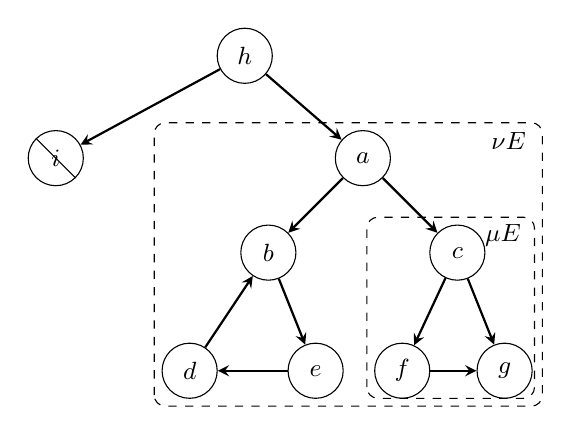
\begin{tikzpicture}[
  >=stealth,
  every node/.style={circle,draw,minimum size=7mm,inner sep=1pt,font=\small},
  edge/.style={->,thick}
]
\node (h) at (0,3.2) {$h$};
\node (i) at (-2.4,1.9) {$i$};
\draw (i.north west)--(i.south east);
\node (a) at (1.5,1.9) {$a$};
\node (b) at (0.3,0.7) {$b$};
\node (c) at (2.7,0.7) {$c$};
\node (d) at (-0.7,-0.8) {$d$};
\node (e) at (0.9,-0.8) {$e$};
\node (f) at (2.0,-0.8) {$f$};
\node (g) at (3.3,-0.8) {$g$};
\draw[edge] (h)--(i);
\draw[edge] (h)--(a);
\draw[edge] (a)--(b);
\draw[edge] (a)--(c);
\draw[edge] (d)--(b);
\draw[edge] (b)--(e);
\draw[edge] (e)--(d);
\draw[edge] (c)--(f);
\draw[edge] (c)--(g);
\draw[edge] (f)--(g);
\draw[dashed,rounded corners] (-1.15,-1.25) rectangle (3.78,2.35);
\node[draw=none,rectangle] at (3.35,2.12) {$\nu E$};
\draw[dashed,rounded corners] (1.55,-1.15) rectangle (3.68,1.15);
\node[draw=none,rectangle] at (3.28,0.92) {$\mu E$};
\end{tikzpicture}
\caption{支持函数示例}
\label{fig:21-2}
\end{figure}

\begin{exercise}[\(\star\)]
\label{ex:21.5.4}
像\cref{exm:21.1.3}那样，给出与\cref{fig:21-2}对应的推导规则。验证
\(E(\{b,c\})=\{g,a,d\}\)、\(E(\{a,i\})=\{g,h\}\)，并验证图中标出的
\(\mu E\) 与 \(\nu E\) 确实分别为最小、最大不动点。
\end{exercise}
\taplauthorsolutionlink{sol:author:21.5.4}{21.5.4}

从支持图可以看出：\(x\in\nu F\) 当且仅当从 \(x\) 出发无法到达任何不受支持
的元素。因此可以枚举从 \(x\) 出发经支持关系可达的全部元素；遇到不受支持
的元素便失败，否则成功。支持图可能含环，枚举过程必须避免陷入无限循环。

\begin{definition}
\label{def:21.5.5}
设 \(F\) 可逆。定义布尔函数 \(\operatorname{gfp}_F\)（简称
\(\operatorname{gfp}\)）：
\[
\operatorname{gfp}(X)=
\begin{cases}
\mathsf{false},&\operatorname{support}(X)\uparrow,\\
\mathsf{true},&\operatorname{support}(X)\subseteq X,\\
\operatorname{gfp}(\operatorname{support}(X)\cup X),&\text{否则}.
\end{cases}
\]
它从 \(X\) 开始不断加入支持集，直到得到 \(F\)-一致集合，或发现不受支持的
元素。
对单个元素约定 \(\operatorname{gfp}(x)=\operatorname{gfp}(\{x\})\)。
\end{definition}

\begin{exercise}[\(\star\)]
\label{ex:21.5.6}
若 \(x\in\nu F\) 位于支持图中的环上，或可到达环上的元素，则
\(x\notin\mu F\)。逆命题是否成立？也就是说，若
\(x\in\nu F\setminus\mu F\)，\(x\) 是否必能到达某个环？
\end{exercise}
\taplauthorsolutionlink{sol:author:21.5.6}{21.5.6}

本节余下部分证明 \(\operatorname{gfp}\) 的正确性与终止性；初次阅读可以直接
跳到下一节。先说明支持函数的两项性质。

\begin{lemma}
\label{lem:21.5.7}
\[
X\subseteq F(Y)\quad\Longleftrightarrow\quad
\operatorname{support}_F(X)\downarrow
\text{ 且 }\operatorname{support}_F(X)\subseteq Y.
\]
\end{lemma}

\begin{proof}
只需对单个 \(x\) 证明。若 \(x\in F(Y)\)，则 \(Y\in\mathcal G_x\)，故
\(\mathcal G_x\ne\varnothing\)。可逆性保证最小生成集
\(\operatorname{support}(x)\) 存在，且包含于 \(Y\)。反过来，若
\(\operatorname{support}(x)\subseteq Y\)，单调性给出
\(F(\operatorname{support}(x))\subseteq F(Y)\)；而支持集的定义保证
\(x\in F(\operatorname{support}(x))\)，所以 \(x\in F(Y)\)。
\end{proof}

\begin{lemma}
\label{lem:21.5.8}
若 \(P\) 是 \(F\) 的不动点，则
\[
X\subseteq P\quad\Longleftrightarrow\quad
\operatorname{support}_F(X)\downarrow
\text{ 且 }\operatorname{support}_F(X)\subseteq P.
\]
\end{lemma}

\begin{proof}
由 \(P=F(P)\) 和\cref{lem:21.5.7}立即得到。
\end{proof}

先证明 \(\operatorname{gfp}\) 的部分正确性；此时尚不保证算法总会终止。

\taplstatementliststart
\begin{theorem}
\label{thm:21.5.9}
\taplstatementlistbreak
\begin{enumerate}
  \item 若 \(\operatorname{gfp}_F(X)=\mathsf{true}\)，则 \(X\subseteq\nu F\)；
  \item 若 \(\operatorname{gfp}_F(X)=\mathsf{false}\)，则 \(X\not\subseteq\nu F\)。
\end{enumerate}
\end{theorem}

\begin{proof}
两项都对一次算法运行的递归结构作归纳。

若算法因 \(\operatorname{support}(X)\subseteq X\) 返回真，
\cref{lem:21.5.7}给出 \(X\subseteq F(X)\)，所以 \(X\) 是 \(F\)-一致的，
余归纳原理给出 \(X\subseteq\nu F\)。若递归调用
\(\operatorname{gfp}(\operatorname{support}(X)\cup X)\) 返回真，归纳假设
给出 \(\operatorname{support}(X)\cup X\subseteq\nu F\)，结论同样成立。

若算法因 \(\operatorname{support}(X)\uparrow\) 返回假，
\cref{lem:21.5.8}给出 \(X\not\subseteq\nu F\)。若递归调用返回假，归纳假设
说明 \(\operatorname{support}(X)\cup X\not\subseteq\nu F\)，即 \(X\) 或其
支持集不包含于 \(\nu F\)；后一种情况再由\cref{lem:21.5.8}推出
\(X\not\subseteq\nu F\)。
\end{proof}

下面给出保证算法终止的一项充分条件。

\begin{definition}
\label{def:21.5.10}
对可逆生成函数 \(F\) 和 \(x\in U\)，定义 \(x\) 的直接前驱集合
\[
\operatorname{pred}_F(x)=
\begin{cases}
\varnothing,&\operatorname{support}_F(x)\uparrow,\\
\operatorname{support}_F(x),&\operatorname{support}_F(x)\downarrow,
\end{cases}
\qquad
\operatorname{pred}_F(X)=\bigcup_{x\in X}\operatorname{pred}_F(x).
\]
从 \(X\) 沿支持关系可达的全部元素组成
\[
\operatorname{reachable}_F(X)=
\bigcup_{n\ge0}\operatorname{pred}_F^n(X),
\qquad
\operatorname{reachable}_F(x)=\operatorname{reachable}_F(\{x\}).
\]
若 \(y\in\operatorname{reachable}_F(x)\)，便称 \(y\) 从 \(x\) 可达。
\end{definition}

\begin{definition}
\label{def:21.5.11}
若每个 \(x\in U\) 的 \(\operatorname{reachable}_F(x)\) 都有限，则称可逆生成
函数 \(F\) 为\termfirst{有限状态的}{finite state}。
\end{definition}

\begin{theorem}
\label{thm:21.5.12}
若 \(\operatorname{reachable}_F(X)\) 有限，则 \(\operatorname{gfp}_F(X)\)
有定义。因而，若 \(F\) 是有限状态的，则算法对任意有限 \(X\subseteq U\) 都终止。
\end{theorem}

\begin{proof}
从初始调用 \(\operatorname{gfp}(X)\) 产生的每次递归调用
\(\operatorname{gfp}(Y)\)，都满足
\(Y\subseteq\operatorname{reachable}(X)\)。每次继续递归时，都会向 \(Y\)
加入至少一个此前尚未包含的可达元素，使下一次调用的参数集合严格包含 \(Y\)。
由于可达集有限，
\[
m(Y)=|\operatorname{reachable}(X)|-|Y|
\]
是严格递减且非负的终止度量。
\end{proof}

\Needspace{9\baselineskip}
\translatornote{对递归调用次数归纳可知，每次调用的参数集合 \(Y\) 都包含于
\(\operatorname{reachable}(X)\)：初始参数就是 \(X\)，而从可达元素再沿一条
支持边得到的元素仍然可达。算法只有在
\(\operatorname{support}(Y)\nsubseteq Y\) 时才会继续递归。此时存在
\(z\in\operatorname{support}(Y)\setminus Y\)，所以下一次调用的参数
\[
Y'=Y\cup\operatorname{support}(Y)
\]
满足 \(Y\subsetneq Y'\)。这样，全部递归参数都被限制在有限集合内，每次递归
却又至少加入一个新元素，因而不可能无限递归。}

\begin{exercise}[\(\star\star\star\)]
\label{ex:21.5.13}
设 \(F\) 可逆，定义
\[
\operatorname{lfp}(X)=
\begin{cases}
\mathsf{false},&\operatorname{support}(X)\uparrow,\\
\mathsf{true},&X=\varnothing,\\
\operatorname{lfp}(\operatorname{support}(X)),&\text{否则}.
\end{cases}
\]
它从 \(X\) 开始沿支持关系缩减集合，直至集合为空。证明该算法部分正确：
\begin{enumerate}
  \item 若 \(\operatorname{lfp}_F(X)=\mathsf{true}\)，则 \(X\subseteq\mu F\)；
  \item 若 \(\operatorname{lfp}_F(X)=\mathsf{false}\)，则 \(X\not\subseteq\mu F\)。
\end{enumerate}
再找出一类生成函数，使 \(\operatorname{lfp}_F\) 对所有有限输入都保证终止。
\end{exercise}
\taplauthorsolutionlink{sol:author:21.5.13}{21.5.13}

\section{更高效的算法}
\label{sec:21.6}

上一节的 \(\operatorname{gfp}\) 每次递归都会重新计算整个集合的支持集。例如，
对\cref{fig:21-2}的 \(E\) 有
\[
\begin{aligned}
\operatorname{gfp}(\{a\})
&=\operatorname{gfp}(\{a,b,c\})\\
&=\operatorname{gfp}(\{a,b,c,e,f,g\})\\
&=\operatorname{gfp}(\{a,b,c,e,f,g,d\})\\
&=\mathsf{true},
\end{aligned}
\]
其中 \(\operatorname{support}(a)\) 被重复计算四次。可以用假设集 \(A\) 记录
已经检查过支持集的元素，用目标集 \(X\) 记录尚待检查的元素。

\begin{definition}
\label{def:21.6.1}
设 \(F\) 可逆，定义函数 \(\operatorname{gfp}_F^a\)，其中上标 \(a\) 表示
assumptions：
\[
\operatorname{gfp}^a(A,X)=
\begin{cases}
\mathsf{false},&\operatorname{support}(X)\uparrow,\\
\mathsf{true},&X=\varnothing,\\
\operatorname{gfp}^a(A\cup X,
  \operatorname{support}(X)\setminus(A\cup X)),&\text{否则}.
\end{cases}
\]
检查 \(x\in\nu F\) 时计算 \(\operatorname{gfp}^a(\varnothing,\{x\})\)。
\end{definition}

该算法以及本节后面的两个算法，都至多计算每个元素的支持集一次。上例的运行
轨迹为
\[
\begin{aligned}
\operatorname{gfp}^a(\varnothing,\{a\})
&=\operatorname{gfp}^a(\{a\},\{b,c\})\\
&=\operatorname{gfp}^a(\{a,b,c\},\{e,f,g\})\\
&=\operatorname{gfp}^a(\{a,b,c,e,f,g\},\{d\})\\
&=\operatorname{gfp}^a(\{a,b,c,e,f,g,d\},\varnothing)\\
&=\mathsf{true}.
\end{aligned}
\]

\taplstatementliststart
\begin{theorem}
\label{thm:21.6.2}
\taplstatementlistbreak
\begin{enumerate}
  \item 若 \(\operatorname{support}_F(A)\subseteq A\cup X\) 且
        \(\operatorname{gfp}_F^a(A,X)=\mathsf{true}\)，则
        \(A\cup X\subseteq\nu F\)；
  \item 若 \(\operatorname{gfp}_F^a(A,X)=\mathsf{false}\)，则
        \(X\not\subseteq\nu F\)。
\end{enumerate}
\end{theorem}

\begin{proof}
与\cref{thm:21.5.9}相似。
\end{proof}

\translatornote{条件
\(\operatorname{support}_F(A)\subseteq A\cup X\) 表示：已检查元素的每项
依赖，要么已经检查过而属于 \(A\)，要么已经列入待检查集合 \(X\)。例如，若
\(A=\{a,b\}\)、\(X=\{c\}\)，而
\(\operatorname{support}_F(a)=\{b,c\}\)、
\(\operatorname{support}_F(b)=\{a\}\)，则
\(\operatorname{support}_F(A)=\{a,b,c\}\subseteq A\cup X\)：\(a\) 依赖的
\(b\) 已经检查过，\(c\) 尚未检查但已经列入 \(X\)，\(b\) 依赖的 \(a\)
也已经检查过。

标准初始调用 \(\operatorname{gfp}^a(\varnothing,\{x\})\) 满足该条件。若某次
调用满足它，下一次调用的参数为
\[
A'=A\cup X,\qquad
X'=\operatorname{support}_F(X)\setminus(A\cup X).
\]
这一定义把当前待检查元素 \(X\) 全部移入已检查集合 \(A'\)，再把它们尚未
处理的依赖放入新的待检查集合 \(X'\)。原有条件给出
\(\operatorname{support}_F(A)\subseteq A'=A\cup X\)；而按照 \(X'\) 的定义，
\(\operatorname{support}_F(X)\) 中的每个元素或者已经属于 \(A'\)，或者属于
\(X'\)。因此
\[
\operatorname{support}_F(A')
=\operatorname{support}_F(A)\cup\operatorname{support}_F(X)
\subseteq A'\cup X'
\]
其中等号来自 \(A'=A\cup X\)。这就说明递归进入下一轮后，同一条件仍然成立。
定理允许用一般的 \(A,X\) 调用算法，所以必须
显式写出这一条件；否则，若 \(X=\varnothing\)，算法会立即返回真，即使
\(A\) 的某项依赖既不在 \(A\) 中，也未列入 \(X\)。}

本节余下部分给出两个更接近常见递归子类型算法的变体；初次阅读可以跳到下一节。

\begin{definition}
\label{def:21.6.3}
算法 \(\operatorname{gfp}^s\) 每次只从 \(X\) 中取一个元素并展开其支持集，
其中上标 \(s\) 表示 single：
\[
\operatorname{gfp}^s(A,X)=
\begin{cases}
\mathsf{true},&X=\varnothing,\\
\operatorname{gfp}^s(A,X\setminus\{x\}),&x\in A,\\
\mathsf{false},&x\notin A\text{ 且 }\operatorname{support}(x)\uparrow,\\
\operatorname{gfp}^s(A\cup\{x\},
  (X\cup\operatorname{support}(x))\setminus(A\cup\{x\})),&\text{否则},
\end{cases}
\]
其中在 \(X\ne\varnothing\) 的分支任取 \(x\in X\)。其正确性不变量与
\cref{thm:21.6.2}完全相同。
\end{definition}

许多现有递归子类型算法一次只接收一个候选元素，而不是候选集合。再作一次小改动
即可得到这种形式。新算法不再尾递归，因为调用栈负责记住尚未检查的子目标；它
同时把假设集 \(A\) 作为参数，并把更新后的假设集作为结果，从而复用已经完成的
递归调用所发现的假设。假设集就这样贯穿整个调用图，因此算法记作
\(\operatorname{gfp}^t\)。\footnote{尾递归调用（或尾调用）是调用者函数执行的
最后一个动作；也就是说，递归调用返回的结果会直接成为调用者的结果。尾调用之所以
值得注意，是因为多数函数式语言编译器会把它实现为一次简单跳转：复用调用者的栈
空间，而不为递归调用分配新的栈帧。因此，以尾递归函数实现的循环可以编译成与等价的
\texttt{while} 循环相同的机器代码。}

\begin{definition}
\label{def:21.6.4}
设 \(F\) 可逆，定义
\[
\operatorname{gfp}^t(A,x)=
\begin{cases}
A,&x\in A,\\
\mathsf{fail},&\operatorname{support}(x)\uparrow,\\
A_n,&\text{否则},
\end{cases}
\]
最后一项中的 \(A_n\) 依次计算如下：
\[
\begin{gathered}
\{x_1,\ldots,x_n\}=\operatorname{support}(x),\qquad
A_0=A\cup\{x\},\\
A_1=\operatorname{gfp}^t(A_0,x_1),\quad\ldots,\quad
A_n=\operatorname{gfp}^t(A_{n-1},x_n).
\end{gathered}
\]
检查 \(x\in\nu F\) 时计算 \(\operatorname{gfp}^t(\varnothing,x)\)：调用成功
表示属于，失败表示不属于。上述顺序计算还约定失败自动向外传播：若某一步递归调用
失败，后续步骤便不再执行，整个调用也返回失败。采用这一约定后，就不必在每次递归
调用旁重复写出失败处理。
\end{definition}

\translatornote{判断递归调用是否处于尾位置，关键不在于它是否写在最后一行，
而在于调用返回后，当前函数是否还有工作要做。粗略地说，
\texttt{return f(y)} 中的调用是尾调用，因为 \texttt{f(y)} 的结果会直接成为
当前函数的结果；\texttt{return 1 + f(y)} 中的调用则不是，因为
\texttt{f(y)} 返回后还要执行加法。从上式可以看出本算法为何不是尾递归：计算出
\(A_1=\operatorname{gfp}^t(A_0,x_1)\) 后，当前调用还要用返回的 \(A_1\)
继续检查 \(x_2\)；得到 \(A_2\) 后还要继续检查 \(x_3\)，依此类推。因此，
对 \(x_i\) 的递归调用返回后，调用者仍有后续工作，不能把它的结果直接作为自身的
结果返回；尚未检查的 \(x_{i+1},\ldots,x_n\) 便由调用栈暂时记住。}

由于该算法不是尾递归，正确性陈述还要加入一个“栈”集合 \(X\)，表示支持集尚待
检查的元素。

\taplstatementliststart
\begin{lemma}
\label{lem:21.6.5}
\taplstatementlistbreak
\begin{enumerate}
  \item 若 \(\operatorname{gfp}_F^t(A,x)=A'\)，则
        \(A\cup\{x\}\subseteq A'\)；
  \item 对任意 \(X\)，若
        \(\operatorname{support}_F(A)\subseteq A\cup X\cup\{x\}\) 且
        \(\operatorname{gfp}_F^t(A,x)=A'\)，则
        \(\operatorname{support}_F(A')\subseteq A'\cup X\)。
\end{enumerate}
\end{lemma}

\translatornote{第 1 项说明，算法成功运行时只会扩充假设集：原有的 \(A\)
不会丢失，当前检查的 \(x\) 也会被加入结果 \(A'\)。第 2 项说明，算法完成后仍
保持同一个关键条件：结果集合中各元素的依赖，要么已经收入结果集合 \(A'\)，
要么仍由调用栈中的待检查集合 \(X\) 负责。}

\begin{proof}
两项都对算法成功运行时形成的递归调用结构作归纳。

先证第 1 项。若 \(x\in A\)，算法直接返回 \(A'=A\)，而
\(A\cup\{x\}=A\)。否则，由算法成功返回 \(A'\) 可知
\(\operatorname{support}(x)\) 有定义。设
\(\operatorname{support}(x)=\{x_1,\ldots,x_n\}\)。算法先令
\(A_0=A\cup\{x\}\)，再依次计算
\(A_i=\operatorname{gfp}^t(A_{i-1},x_i)\)，最后返回 \(A'=A_n\)。对每个较小的
递归调用应用第 1 项的归纳假设，可知 \(A_{i-1}\subseteq A_i\)。因此
\(A\cup\{x\}=A_0\subseteq A_n=A'\)。

再证第 2 项。任取 \(X_0\)，并假设
\[
\operatorname{support}(A)\subseteq A\cup X_0\cup\{x\}
\]
若 \(x\in A\)，算法返回 \(A'=A\)；此时 \(\{x\}\subseteq A\)，所以上述前提
立即给出 \(\operatorname{support}(A')\subseteq A'\cup X_0\)。

先讨论 \(\operatorname{support}(x)=\{x_1,x_2\}\) 的情形。算法依次计算
\[
\begin{gathered}
A_0=A\cup\{x\},\qquad
A_1=\operatorname{gfp}^t(A_0,x_1),\qquad
A_2=\operatorname{gfp}^t(A_1,x_2)
\end{gathered}
\]
并返回 \(A'=A_2\)。证明的关键是依次对这两次递归调用使用归纳假设：处理
\(x_1\) 时，尚未处理的 \(x_2\) 仍须列入待检查集合；处理 \(x_2\) 时，它本身
成为当前检查的元素，待检查集合便恢复为 \(X_0\)。

具体而言，令 \(X_1=X_0\cup\{x_2\}\)。为了把归纳假设应用于
\(A_1=\operatorname{gfp}^t(A_0,x_1)\)，需要先验证
\(\operatorname{support}(A_0)\subseteq A_0\cup X_1\cup\{x_1\}\)。这由
\[
\begin{aligned}
\operatorname{support}(A_0)
&=\operatorname{support}(A)\cup\operatorname{support}(x)\\
&=\operatorname{support}(A)\cup\{x_1,x_2\}\\
&\subseteq A\cup\{x\}\cup X_0\cup\{x_1,x_2\}\\
&=A_0\cup X_1\cup\{x_1\}
\end{aligned}
\]
得到。于是，第 2 项的归纳假设给出
\[
\operatorname{support}(A_1)
\subseteq A_1\cup X_1
=A_1\cup X_0\cup\{x_2\}
\]
这正是把归纳假设应用于
\(A_2=\operatorname{gfp}^t(A_1,x_2)\) 时所需的前提，其中引理中的辅助集合
\(X\) 取为 \(X_0\)。因此
\[
\operatorname{support}(A_2)\subseteq A_2\cup X_0
\]
又因 \(A'=A_2\)，结论成立。

若 \(\operatorname{support}(x)\) 含有任意有限个元素，论证完全相同：依次处理
\(x_i\) 时，把 \(x_{i+1},\ldots,x_n\) 与 \(X_0\) 一同视为尚待检查的元素。
形式上对支持集大小作内层归纳，即得一般结论。
\end{proof}

\taplstatementliststart
\begin{theorem}
\label{thm:21.6.6}
\taplstatementlistbreak
\begin{enumerate}
  \item 若 \(\operatorname{gfp}_F^t(\varnothing,x)=A'\)，则 \(x\in\nu F\)；
  \item 若 \(\operatorname{gfp}_F^t(\varnothing,x)=\mathsf{fail}\)，则
        \(x\notin\nu F\)。
\end{enumerate}
\end{theorem}

\begin{proof}
第 1 项中，\cref{lem:21.6.5}第 1 项给出 \(x\in A'\)；再把第 2 项的
\(X\) 取为空集，得到
\(\operatorname{support}(A')\subseteq A'\)，所以 \(A'\) 是
\(F\)-一致的，余归纳原理给出 \(A'\subseteq\nu F\)。第 2 项对失败运行的
深度作归纳，并使用\cref{lem:21.5.8}。
\end{proof}

\translatornote{第 2 项的归纳论证可以展开如下。先把结论加强为：对任意假设集
\(A\)，若 \(\operatorname{gfp}_F^t(A,x)=\mathsf{fail}\)，则
\(x\notin\nu F\)；再对这次失败运行的递归深度作归纳。由于 \(\nu F\) 是
\(F\) 的不动点，\cref{lem:21.5.8}对单个元素给出
\[
x\in\nu F
\quad\Longleftrightarrow\quad
\operatorname{support}_F(x)\downarrow
\text{ 且 }\operatorname{support}_F(x)\subseteq\nu F
\]
若当前调用因 \(\operatorname{support}_F(x)\uparrow\) 直接失败，上式立即说明
\(x\notin\nu F\)。否则，失败来自某次较小的递归调用
\(\operatorname{gfp}_F^t(A_{i-1},x_i)=\mathsf{fail}\)，其中
\(x_i\in\operatorname{support}_F(x)\)。归纳假设给出
\(x_i\notin\nu F\)，因而
\(\operatorname{support}_F(x)\nsubseteq\nu F\)；再次使用上述等价关系，即得
\(x\notin\nu F\)。也就是说，最深处的不受支持元素先被判定为不属于
\(\nu F\)，此结论再沿失败的调用栈逐层向外传递。最后取 \(A=\varnothing\)，
便得到定理第 2 项。}

本节所有算法都会检查可达集，因此，只要 \(F\) 是有限状态的，它们便会对所有输入
终止。

\section{正则树}
\label{sec:21.7}

至此，我们已经为如下问题给出了通用算法：若一个集合被定义为生成函数 \(F\) 的
最大不动点，怎样判断给定元素是否属于这个集合；这里假定 \(F\) 可逆且具有有限状态。
另一方面，我们已经把无限树之间的子类型关系定义为特定生成函数 \(\mathcal S\) 的
最大不动点。接下来要做的很明确：把 \(\mathcal S\) 代入前述算法，得到具体的子类型
检查算法。当然，这一算法不会对所有输入都终止，因为从一对无限类型出发能够到达的
状态一般可能有无穷多个。不过本节将会看到，若把讨论限制在某种性质良好的无限类型，
即所谓的\termfirst{正则类型}{regular type}上，可达状态集合便一定有限，子类型检查
算法也必然终止。

\begin{definition}
\label{def:21.7.1}
若存在路径 \(\pi\)，使
\[
S=\lambda\sigma.\,T(\pi,\sigma),
\]
则称树类型 \(S\) 是树类型 \(T\) 的子树。换句话说，把树看作从路径到符号的
函数时，\(S\) 是在传给 \(T\) 的路径参数前加上固定前缀 \(\pi\) 得到的。
这个前缀是从 \(T\) 的根到 \(S\) 的根的路径。\(T\) 的全部子树组成的集合记作
\(\operatorname{subtrees}(T)\)。
\end{definition}

\begin{definition}
\label{def:21.7.2}
若 \(\operatorname{subtrees}(T)\) 有限，则称树类型 \(T\) 正则。全部正则树
类型的集合记作 \(\mathcal T_r\)。
\end{definition}

\taplstatementliststart
\begin{example}
\label{exm:21.7.3}
\taplstatementlistbreak
\begin{enumerate}
  \item 每个有限树类型都正则；不同子树的数量不超过节点数。例如
        \(T=\tapltype{Top}\to(\tapltype{Top}\times\tapltype{Top})\)
        有五个节点，却只有 \(T\) 自身、
        \(\tapltype{Top}\times\tapltype{Top}\) 和 \(\tapltype{Top}\) 三棵
        不同子树。
  \item 有些无限树也是正则的。例如
        \(T=\tapltype{Top}\times(\tapltype{Top}\times
        (\tapltype{Top}\times\cdots))\) 只有 \(T\) 自身和
        \(\tapltype{Top}\) 两棵不同子树。
  \item 树
        \[
        T=B\times(A\times(B\times(A\times(A\times
          (B\times(A\times(A\times(A\times(B\times\cdots)))))))))
        \]
        中，相邻的 \(B\) 之间依次夹着越来越多个 \(A\)，因此它不正则。证明
        \(T\subtype T\) 所需的可达子类型对也会有无限多个。
\end{enumerate}
\end{example}

\Needspace{8\baselineskip}
\begin{proposition}
\label{prop:21.7.4}
把生成函数 \(\mathcal S\) 的作用范围限定为正则树类型后，所得的生成函数
\(\mathcal S_r\) 是有限状态的。
\end{proposition}

\begin{proof}
对任意正则树类型对 \((S,T)\)，
\[
\operatorname{reachable}_{\mathcal S_r}(S,T)
\subseteq
\bigl(\operatorname{subtrees}(S)\times\operatorname{subtrees}(T)\bigr)
\cup
\bigl(\operatorname{subtrees}(T)\times\operatorname{subtrees}(S)\bigr).
\]
函数参数位置的逆变可能交换有序对的两个分量，因此需要同时包含这两个方向。
两个子树集合都有限，右侧的并集也有限，故左侧有限。
\end{proof}

\translatornote{证明右侧的两个笛卡尔积列出了子类型检查过程中所有可能遇到的
类型对。以检查 \(S_1\to S_2\subtype T_1\to T_2\) 为例，箭头规则接下来要求检查
\(T_1\subtype S_1\) 和 \(S_2\subtype T_2\)：参数位置因逆变而交换方向，
结果位置则保持原方向。因此，后续遇到的类型对只可能落在证明所列的两个笛卡尔积
中。正则树虽然可以无限展开，却只有有限多棵互不相同的子树，所以这样的类型对
只有有限多个；实现只要记住已经检查过的类型对，便不会因循环而无限递归。}

因此，把成员关系算法用于 \(\mathcal S_r\)，就得到正则树类型子类型关系的判定
过程。实际实现还需要有限结构来表示正则树；下一节介绍一种这样的结构，即
\(\mu\)-记法。

\section{\texorpdfstring{\(\mu\)-类型}{μ-类型}}
\label{sec:21.8}

本节给出有限的 \(\mu\)-记法，定义 \(\mu\)-表达式上的子类型关系，并证明它与
树类型上的子类型关系相对应。

\begin{definition}
\label{def:21.8.1}
预先固定一列类型变量名 \(X_1,X_2,\ldots\)，并用 \(X\) 表示其中任意一个。
\termfirst{原始 \(\mu\)-类型}{raw \(\mu\)-type}由以下文法生成：
\[
T ::= X\mid\tapltype{Top}\mid T\times T\mid T\to T\mid\mu X.T
\]
全部原始 \(\mu\)-类型的集合记作 \(\mathcal T_m^{\mathrm{raw}}\)。在
\(\mu X.T\) 中，\(\mu X\) 绑定后面类型表达式 \(T\) 中出现的 \(X\)，其作用
与 lambda 抽象中的变量绑定相同。因此，我们可以区分类型中的自由变量与受约束
变量，并把不含自由变量的原始 \(\mu\)-类型称为闭类型。两个原始 \(\mu\)-类型
如果只在受约束变量的名称上不同，就视为相同。\(\operatorname{FV}(T)\) 表示
\(T\) 中自由变量的集合；\([X\mapsto S]T\) 表示把 \(T\) 中 \(X\) 的所有自由
出现替换为 \(S\)。替换时若可能发生变量捕获，就先对相应的受约束变量重命名。
\end{definition}

为了让原始 \(\mu\)-类型与正则树严格对应，还需排除某些特殊写法。我们希望反复
展开 \(\mu\)-绑定后，能够逐层看到由 \(\tapltype{Top}\)、\(\times\) 或 \(\to\)
标记的树节点；但 \(\mu X.X\) 展开后仍是自身，无论展开多少次，根节点都不会
显露出来。一般地，问题来自形如
\(\mu X.\mu X_1\cdots\mu X_n.X\) 的子表达式，其中
\(X_1,\ldots,X_n\) 均不同于 \(X\)。

\begin{definition}
\label{def:21.8.2}
若对原始 \(\mu\)-类型 \(T\) 的每个子表达式
\(\mu X.\mu X_1\cdots\mu X_n.S\)，都有 \(S\ne X\)，则称 \(T\) 是
\termfirst{收缩的}{contractive}。等价地说，对每个由 \(\mu\) 绑定的变量
\(X\)，从相应的 \(\mu X\) 沿语法树走到由它绑定的任意一次 \(X\) 出现，途中
至少要经过一个 \(\to\) 或 \(\times\) 节点。

下文把收缩的原始 \(\mu\)-类型简称为 \(\mu\)-类型，其集合记作
\(\mathcal T_m\)。把从 \(T\) 最外层开始连续嵌套的 \(\mu\) 绑定数量记作
\(\mu\text{-}\operatorname{height}(T)\)。
\end{definition}

\begin{definition}
\label{def:21.8.3}
把闭 \(\mu\)-类型映射到树类型的函数
\(\operatorname{treeof}\) 归纳定义如下（\(i\in\{1,2\}\)）：
\[
\begin{aligned}
\operatorname{treeof}(\tapltype{Top})(\epsilon)
  &=\tapltype{Top}\\
\operatorname{treeof}(T_1\to T_2)(\epsilon)
  &=\to\\
\operatorname{treeof}(T_1\to T_2)(i,\pi)
  &=\operatorname{treeof}(T_i)(\pi)\\
\operatorname{treeof}(T_1\times T_2)(\epsilon)
  &=\times\\
\operatorname{treeof}(T_1\times T_2)(i,\pi)
  &=\operatorname{treeof}(T_i)(\pi)\\
\operatorname{treeof}(\mu X.T)(\pi)
  &=\operatorname{treeof}([X\mapsto\mu X.T]T)(\pi)
\end{aligned}
\]
\end{definition}

\(\operatorname{treeof}(T)(\pi)\) 的计算只展开类型 \(T\) 中沿有限路径
\(\pi\) 经过的部分，并返回路径终点处的标签，即 \(\tapltype{Top}\)、\(\to\)
或 \(\times\)。对任意闭 \(\mu\)-类型 \(T\) 和有限路径 \(\pi\)，这一计算都有
定义且会终止。右侧每次递归调用都会严格减小字典序数对
\((|\pi|,\mu\text{-}\operatorname{height}(T))\)：箭头和积类型分支减小路径长度，
\(\mu X.T\) 分支保持路径长度，却使类型参数开头连续出现的 \(\mu\) 绑定数量
严格减小。所有调用也都
保持参数类型的收缩性与闭性；特别是，\(\mu X.T\) 收缩且闭，当且仅当它的展开
\([X\mapsto\mu X.T]T\) 也收缩且闭。

约定
\(\operatorname{treeof}(S,T)=(\operatorname{treeof}(S),
\operatorname{treeof}(T))\)。\cref{fig:21-3}展示一个展开示例。

\begin{figure}[!ht]
\centering
\begin{tikzpicture}[
  level distance=11mm,
  level 1/.style={sibling distance=38mm},
  level 2/.style={sibling distance=23mm},
  level 3/.style={sibling distance=16mm},
  every node/.style={font=\small}
]
\node {$\to$}
  child {node {$\times$}
    child {node {$\to$}
      child {node {$\times$}
        child {node {$\vdots$}}
        child {node {$\tapltype{Top}$}}}
      child {node {$\vdots$}}}
    child {node {$\tapltype{Top}$}}}
  child {node {$\to$}
    child {node {$\times$}
      child {node {$\vdots$}}
      child {node {$\tapltype{Top}$}}}
    child {node {$\vdots$}}};
\end{tikzpicture}
\caption{\(\operatorname{treeof}(\mu X.((X\times\tapltype{Top})\to X))\) 的展开}
\label{fig:21-3}
\end{figure}

树类型的子类型关系是 \(\mathcal S\) 的最大不动点。现在把语法扩展到
\(\mu\)-类型，其行为可由左右 \(\mu\)-折叠规则描述：
\[
\frac{S\subtype[X\mapsto\mu X.T]T}{S\subtype\mu X.T}
\qquad
\frac{[X\mapsto\mu X.S]S\subtype T}{\mu X.S\subtype T}.
\]

\translatornote{“左”“右”指 \(\mu\)-类型出现在子类型判断符号 \(\subtype\)
的哪一侧。沿推导树从结论向前提读，两条规则分别展开右侧或左侧的递归类型；
反向从前提向结论读，则是把展开形式折叠回 \(\mu\)-类型。}

\begin{definition}
\label{def:21.8.4}
若 \((S,T)\in\nu\mathcal S_\mu\)，则称 \(\mu\)-类型 \(S\) 是 \(T\) 的
子类型，其中
\(\mathcal S_\mu:\powerset(\mathcal T_m\times\mathcal T_m)
\to\powerset(\mathcal T_m\times\mathcal T_m)\) 定义为
\[
\begin{aligned}
\mathcal S_\mu(R)={}&
\{(S,\tapltype{Top})\mid S\in\mathcal T_m\}\\
&\cup\{(S_1\times S_2,T_1\times T_2)
       \mid(S_1,T_1),(S_2,T_2)\in R\}\\
&\cup\{(S_1\to S_2,T_1\to T_2)
       \mid(T_1,S_1),(S_2,T_2)\in R\}\\
&\cup\{(S,\mu X.T)\mid(S,[X\mapsto\mu X.T]T)\in R\}\\
&\cup\{(\mu X.S,T)\mid([X\mapsto\mu X.S]S,T)\in R,\quad
       T\ne\tapltype{Top},\ T\ne\mu Y.T_1\}.
\end{aligned}
\]
\end{definition}

最后两项故意不对称：若两边都以 \(\mu\) 开头，或右边是
\(\tapltype{Top}\)，最后两项原本会重叠；加入条件后，生成函数才可逆。
更自然的声明式生成函数 \(\mathcal S_d\) 与上面的折叠规则逐项对应，下一题
说明它虽不可逆，却生成同一个最大不动点。\footnote{下标 \(d\) 表示该函数来自
声明式（declarative）的 \(\mu\)-折叠规则；\(\mathcal S_\mu\) 则采用算法式
分支。}

\begin{exercise}[\(\star\star\star\)]
\label{ex:21.8.5}
写出 \(\mathcal S_d\)，证明它不可逆，并证明
\(\nu\mathcal S_d=\nu\mathcal S_\mu\)。
\end{exercise}
\taplauthorsolutionlink{sol:author:21.8.5}{21.8.5}

\(\mathcal S_\mu\) 的支持函数为
\[
\operatorname{support}_{\mathcal S_\mu}(S,T)=
\begin{cases}
\varnothing,&T=\tapltype{Top},\\
\{(S_1,T_1),(S_2,T_2)\},
  &S=S_1\times S_2,\ T=T_1\times T_2,\\
\{(T_1,S_1),(S_2,T_2)\},
  &S=S_1\to S_2,\ T=T_1\to T_2,\\
\{(S,[X\mapsto\mu X.T_1]T_1)\},&T=\mu X.T_1,\\
\{([X\mapsto\mu X.S_1]S_1,T)\},
  &S=\mu X.S_1,\ T\ne\mu Y.T_1,\ T\ne\tapltype{Top},\\
\uparrow,&\text{其他情形}.
\end{cases}
\]

还需确认：有限的 \(\mu\)-表示与无限树表示给出的子类型关系确实一致。

\begin{lemma}
\label{lem:21.8.6}
设 \(R\subseteq\mathcal T_m\times\mathcal T_m\) 是
\(\mathcal S_\mu\)-一致的。对任意 \((S,T)\in R\)，存在
\((S',T')\in R\)，使
\(\operatorname{treeof}(S',T')=\operatorname{treeof}(S,T)\)，并且或者
\(T'=\tapltype{Top}\)，或者 \(S'\)、\(T'\) 都不以 \(\mu\) 开头。
\end{lemma}

\begin{proof}
以 \(S\) 与 \(T\) 最外层连续出现的 \(\mu\) 绑定总数为归纳对象。若
\(T=\tapltype{Top}\)，取 \((S',T')=(S,T)\)；若两边都不以 \(\mu\)
开头，也取 \((S',T')=(S,T)\)。

若 \((S,T)=(S,\mu X.T_1)\)，由于 \(R\) 是
\(\mathcal S_\mu\)-一致的，有 \(R\subseteq\mathcal S_\mu(R)\)，故
\[
(S,\mu X.T_1)\in\mathcal S_\mu(R).
\]
根据\cref{def:21.8.4}，右侧以 \(\mu\) 开头的类型对只能由右
\(\mu\)-折叠分支生成。因此
\[
(S,[X\mapsto\mu X.T_1]T_1)\in R.
\]
收缩性保证把右侧的 \(\mu X.T_1\) 展开一层后，所得类型最外层连续出现的
\(\mu\) 绑定恰好少一个，故可应用归纳假设。按照 \(\operatorname{treeof}\)
对递归类型的定义，类型与其展开一层所得的类型表示同一棵无限树，因此这一步
展开不会改变 \(\operatorname{treeof}\) 的结果。

最后考虑左侧以 \(\mu\) 开头的情形。前两种情形已经排除了
\(T=\tapltype{Top}\) 和右侧以 \(\mu\) 开头的情况；此时
\(\mathcal S_\mu\) 的左 \(\mu\)-折叠分支要求展开左侧，并在 \(R\) 中给出
相应的类型对。展开使归纳量减一，余下论证与右侧情形相同。
\end{proof}

\translatornote{原书引理的结论没有列出 \(T'=\tapltype{Top}\) 这一例外。
例如
\(R=\{(\mu X.\tapltype{Top},\tapltype{Top})\}\) 是
\(\mathcal S_\mu\)-一致的，因为 \(\mathcal S_\mu\) 的第一项支持任意
\((S,\tapltype{Top})\)；但 \(R\) 中没有左侧不以 \(\mu\) 开头的类型对。
译文把引理修正为后续定理实际需要的形式：右侧为 \(\tapltype{Top}\) 时直接
处理，其余情形才把两侧展开到都不以 \(\mu\) 开头。}

\begin{theorem}
\label{thm:21.8.7}
对 \((S,T)\in\mathcal T_m\times\mathcal T_m\)，
\[
(S,T)\in\nu\mathcal S_\mu
\quad\Longleftrightarrow\quad
\operatorname{treeof}(S,T)\in\nu\mathcal S
\]
\end{theorem}

\begin{proof}
先证从左到右，即由 \((S,T)\in\nu\mathcal S_\mu\) 推出
\(\operatorname{treeof}(S,T)\in\nu\mathcal S\)。令
\((A,B)=\operatorname{treeof}(S,T)\in\mathcal T\times\mathcal T\)。按照余归纳
原理，只要能找到一个包含 \((A,B)\) 的 \(\mathcal S\)-一致关系
\(Q\subseteq\mathcal T\times\mathcal T\)，结论便成立。取
\[
Q=\operatorname{treeof}(\nu\mathcal S_\mu)
=\{\operatorname{treeof}(S',T')\mid(S',T')\in\nu\mathcal S_\mu\}
\]
这里把 \(\operatorname{treeof}\) 逐元素作用于关系
\(\nu\mathcal S_\mu\) 中的每个类型对。要证明 \(Q\) 是
\(\mathcal S\)-一致的，必须证明：对每个 \((A',B')\in Q\)，都有
\((A',B')\in\mathcal S(Q)\)。

任取 \((A',B')\in Q\)，并选取
\((S',T')\in\nu\mathcal S_\mu\)，使得
\(\operatorname{treeof}(S',T')=(A',B')\)。由\cref{lem:21.8.6}，可以
选择这样的 \((S',T')\)：或者 \(T'=\tapltype{Top}\)，或者 \(S'\) 和
\(T'\) 都不以 \(\mu\) 开头。由于
\(\nu\mathcal S_\mu\) 是 \(\mathcal S_\mu\)-一致的，
\((S',T')\) 必须由 \(\mathcal S_\mu\) 定义中的某一项支持；在上述选择下，
只需讨论以下三种形式。

\textbf{情形：\((S',T')=(S',\tapltype{Top})\)。}
此时 \(B'=\tapltype{Top}\)，由 \(\mathcal S\) 的定义立即得到
\((A',B')\in\mathcal S(Q)\)。

\textbf{情形：}
\[
(S',T')=(S_1\times S_2,T_1\times T_2),
\qquad
(S_1,T_1),(S_2,T_2)\in\nu\mathcal S_\mu
\]
由 \(\operatorname{treeof}\) 的定义，
\(B'=\operatorname{treeof}(T')=B_1\times B_2\)，其中
\(B_i=\operatorname{treeof}(T_i)\)；类似地，
\(A'=A_1\times A_2\)，其中 \(A_i=\operatorname{treeof}(S_i)\)。
分别对上面的两个类型对应用 \(\operatorname{treeof}\)，得到
\[
(A_1,B_1),(A_2,B_2)\in Q
\]
再由 \(\mathcal S\) 的定义可知
\[
(A',B')=(A_1\times A_2,B_1\times B_2)\in\mathcal S(Q)
\]

\textbf{情形：}
\[
(S',T')=(S_1\to S_2,T_1\to T_2),
\qquad
(T_1,S_1),(S_2,T_2)\in\nu\mathcal S_\mu
\]
论证与积类型情形类似；函数参数位置的类型对按逆变方向排列。由此得到
\((A',B')\in\mathcal S(Q)\)。

三种情形都满足要求，故 \(Q\subseteq\mathcal S(Q)\)，即 \(Q\) 是
\(\mathcal S\)-一致的。余归纳原理于是给出
\((A,B)\in\nu\mathcal S\)，从左到右的方向得证。

再证从右到左，即由 \(\operatorname{treeof}(S,T)\in\nu\mathcal S\) 推出
\((S,T)\in\nu\mathcal S_\mu\)。按照余归纳原理，只需找到一个包含
\((S,T)\) 的 \(\mathcal S_\mu\)-一致关系
\(R\subseteq\mathcal T_m\times\mathcal T_m\)。取
\[
R=\{(S',T')\in\mathcal T_m\times\mathcal T_m
\mid\operatorname{treeof}(S',T')\in\nu\mathcal S\}
\]
显然 \((S,T)\in R\)。为了完成证明，还需证明：若
\((S',T')\in R\)，则 \((S',T')\in\mathcal S_\mu(R)\)。

由于 \(\nu\mathcal S\) 是 \(\mathcal S\)-一致的，其中任意类型对
\((A',B')\) 只能具有以下三种形式之一：
\((A',\tapltype{Top})\)、\((A_1\times A_2,B_1\times B_2)\) 或
\((A_1\to A_2,B_1\to B_2)\)。结合
\(\operatorname{treeof}\) 的定义可知，\(R\) 中的任意类型对
\((S',T')\) 必须具有以下五种形式之一：
\((S',\tapltype{Top})\)、\((S_1\times S_2,T_1\times T_2)\)、
\((S_1\to S_2,T_1\to T_2)\)、\((S',\mu X.T_1)\) 或
\((\mu X.S_1,T')\)。下面逐一讨论。

\textbf{情形：\((S',T')=(S',\tapltype{Top})\)。}
由 \(\mathcal S_\mu\) 的定义，立即有
\((S',T')\in\mathcal S_\mu(R)\)。

\textbf{情形：\((S',T')=(S_1\times S_2,T_1\times T_2)\)。}
令 \((A',B')=\operatorname{treeof}(S',T')\)，则
\[
(A',B')=(A_1\times A_2,B_1\times B_2)
\]
其中 \(A_i=\operatorname{treeof}(S_i)\)，
\(B_i=\operatorname{treeof}(T_i)\)。由 \((S',T')\in R\) 的定义可知
\((A',B')\in\nu\mathcal S\)。又因为 \(\nu\mathcal S\) 是
\(\mathcal S\)-一致的，所以
\[
(A_1,B_1),(A_2,B_2)\in\nu\mathcal S
\]
再由 \(R\) 的定义得到 \((S_1,T_1),(S_2,T_2)\in R\)。因此，
\(\mathcal S_\mu\) 定义中的积类型分支给出
\[
(S',T')=(S_1\times S_2,T_1\times T_2)\in\mathcal S_\mu(R)
\]

\textbf{情形：\((S',T')=(S_1\to S_2,T_1\to T_2)\)。}
论证类似；函数参数位置使用反向的类型对 \((T_1,S_1)\)，结果位置使用
\((S_2,T_2)\)。

\textbf{情形：\((S',T')=(S',\mu X.T_1)\)。}
令
\[
T''=[X\mapsto\mu X.T_1]T_1
\]
根据定义，\(\operatorname{treeof}(T'')=\operatorname{treeof}(T')\)。
因此，由 \(R\) 的定义可知 \((S',T'')\in R\)，再由
\(\mathcal S_\mu\) 的定义得到
\((S',T')\in\mathcal S_\mu(R)\)。

\textbf{情形：\((S',T')=(\mu X.S_1,T')\)。}
若 \(T'=\tapltype{Top}\)，则归入第一种情形；若 \(T'\) 也以 \(\mu\)
开头，则归入“右侧为 \(\mu\)-类型”的情形。余下只需考虑 \(T'\) 既不是
\(\tapltype{Top}\)、也不以 \(\mu\) 开头的情况；此时展开左侧的递归类型，
论证与展开右侧时对称。

以上五种情形都给出 \((S',T')\in\mathcal S_\mu(R)\)，故
\(R\subseteq\mathcal S_\mu(R)\)，即 \(R\) 是
\(\mathcal S_\mu\)-一致的。余归纳原理于是给出
\((S,T)\in\nu\mathcal S_\mu\)，从右到左的方向得证。
\end{proof}

该定理表明，\(\mu\)-类型的子类型关系相对于其所表示的无限树子类型关系既可靠
又完备。

\section{子表达式计数}
\label{sec:21.9}

把\cref{def:21.6.4}的一般算法 \(\operatorname{gfp}^t\) 用于
\cref{def:21.8.4}的支持函数，就得到\cref{fig:21-4}的具体子类型算法。
\taplsecref{21.6}{sec:21.6}已经说明，只要
\(\operatorname{reachable}_{\mathcal S_\mu}(S,T)\) 对每对 \(\mu\)-类型
都有限，算法便会终止；本节证明这一点。

\begin{figure}[!ht]
\centering
\begin{minipage}{0.86\linewidth}
\begin{align*}
\operatorname{subtype}(A,S,T)={}&
\begin{cases}
A,&(S,T)\in A,\\
\operatorname{subtype}'(A\cup\{(S,T)\},S,T),&\text{否则},
\end{cases}\\[2pt]
\operatorname{subtype}'(A_0,S,T)={}&
\begin{cases}
A_0,&T=\tapltype{Top},\\
\operatorname{subtype}(A_1,S_2,T_2),
 &\substack{S=S_1\times S_2,\ T=T_1\times T_2,\\
 A_1=\operatorname{subtype}(A_0,S_1,T_1)},\\
\operatorname{subtype}(A_1,S_2,T_2),
 &\substack{S=S_1\to S_2,\ T=T_1\to T_2,\\
 A_1=\operatorname{subtype}(A_0,T_1,S_1)},\\
\operatorname{subtype}(A_0,S,[X\mapsto\mu X.T_1]T_1),
 &T=\mu X.T_1,\\
\operatorname{subtype}(A_0,[X\mapsto\mu X.S_1]S_1,T),
 &S=\mu X.S_1,\\
\mathsf{fail},&\text{其他情形}.
\end{cases}
\end{align*}
\end{minipage}
\caption{\(\mu\)-类型的具体子类型算法}
\label{fig:21-4}
\end{figure}

看起来这几乎显然，严格证明却需要不少工作。困难在于，“闭子表达式”有两种定义。
\termfirst{自顶向下子表达式}{top-down subexpression}正好对应支持函数在展开时
产生的表达式；\termfirst{自底向上子表达式}{bottom-up subexpression}则便于
证明任意闭 \(\mu\)-类型只有有限多个闭子表达式。终止性证明会同时定义二者，
再证明前者包含于后者。以下论证依据 Brandt 与 Henglein（1997）。

\begin{definition}
\label{def:21.9.1}
若 \((S,T)\in\mu\operatorname{TD}\)，则称 \(S\) 是 \(T\) 的自顶向下
子表达式，记作 \(S\sqsubseteq T\)，其中
\[
\begin{aligned}
\operatorname{TD}(R)={}&\{(T,T)\mid T\in\mathcal T_m\}\\
&\cup\{(S,T_1\times T_2)\mid(S,T_1)\in R\}\\
&\cup\{(S,T_1\times T_2)\mid(S,T_2)\in R\}\\
&\cup\{(S,T_1\to T_2)\mid(S,T_1)\in R\}\\
&\cup\{(S,T_1\to T_2)\mid(S,T_2)\in R\}\\
&\cup\{(S,\mu X.T)\mid(S,[X\mapsto\mu X.T]T)\in R\}.
\end{aligned}
\]
\end{definition}

\begin{exercise}[\(\star\)]
\label{ex:21.9.2}
用一组推导规则给出关系 \(S\sqsubseteq T\) 的等价定义。
\end{exercise}
\taplauthorsolutionlink{sol:author:21.9.2}{21.9.2}

\begin{lemma}
\label{lem:21.9.3}
若 \((S',T')\in\operatorname{support}_{\mathcal S_\mu}(S,T)\)，则
\(S'\sqsubseteq S\) 或 \(S'\sqsubseteq T\)，且
\(T'\sqsubseteq S\) 或 \(T'\sqsubseteq T\)。
\end{lemma}

\begin{proof}
逐项检查 \(\operatorname{support}_{\mathcal S_\mu}\) 的定义即可。
\end{proof}

\translatornote{本引理说明，支持函数从 \((S,T)\) 产生下一批待检查类型对时，
其中的类型都来自原输入 \(S\) 或 \(T\) 的自顶向下子表达式，不会凭空出现
新的类型。积类型分支产生的 \((S_i,T_i)\) 分别来自 \(S\) 和 \(T\)；箭头
类型的参数位置逆变，产生的依赖项为 \((T_1,S_1)\)，左右来源会交换，因此
结论必须写成“是 \(S\) 或 \(T\) 的子表达式”，不能固定对应哪一侧。递归
类型分支只是把一侧展开一层，而展开所得类型也属于原递归类型的自顶向下
子表达式。这个结论随后用于证明：算法从初始类型对出发能够到达的所有类型，
都受原输入子表达式集合的限制。}

\begin{lemma}
\label{lem:21.9.4}
若 \(S\sqsubseteq U\) 且 \(U\sqsubseteq T\)，则 \(S\sqsubseteq T\)。
\end{lemma}

\begin{proof}
令
\[
R=\{(U,T)\mid\forall S.\ S\sqsubseteq U\Rightarrow S\sqsubseteq T\}
\]
要证 \(\mu\operatorname{TD}\subseteq R\)。依归纳原理，只需证明
\(R\) 对 \(\operatorname{TD}\) 闭合，即
\(\operatorname{TD}(R)\subseteq R\)。任取
\((U,T)\in\operatorname{TD}(R)\)，按照它由
\(\operatorname{TD}\) 定义中的哪一项生成，分类讨论。若当前类型对由
“每个类型都是自身的子表达式”这一分支生成，即 \(U=T\)，结论直接成立。
若当前类型对由积类型的左分支生成，则
\(T=T_1\times T_2\) 且 \((U,T_1)\in R\)。要证明当前类型对
\((U,T_1\times T_2)\) 也属于 \(R\)，任取 \(S\sqsubseteq U\)；由
\((U,T_1)\in R\) 的定义先有 \(S\sqsubseteq T_1\)，再由
\(\operatorname{TD}\) 的积类型分支得到 \(S\sqsubseteq T_1\times T_2\)。
其他分支相同。
\end{proof}

\translatornote{本引理要证明：只要 \(S\sqsubseteq U\) 且
\(U\sqsubseteq T\)，就有 \(S\sqsubseteq T\)。作者把待证结论编码进关系
\[
R=\{(U,T)\mid\forall S.\ S\sqsubseteq U\Rightarrow S\sqsubseteq T\}
\]
按照这个定义，\((U,T)\in R\) 表示 \(U\) 的每个子表达式也都是 \(T\) 的
子表达式。因此，只要证明每个满足 \(U\sqsubseteq T\) 的类型对都属于 \(R\)，
也就是证明
\[
\mu\operatorname{TD}\subseteq R
\]
便能立即得到传递性：已知 \(U\sqsubseteq T\)，即
\((U,T)\in\mu\operatorname{TD}\)，上述包含关系给出 \((U,T)\in R\)；再按
\(R\) 的定义，已知 \(S\sqsubseteq U\) 时便有 \(S\sqsubseteq T\)。

还需说明为什么证明 \(R\) 对 \(\operatorname{TD}\) 闭合就足够。
\(\mu\operatorname{TD}\) 是对 \(\operatorname{TD}\) 的生成规则闭合的最小
关系；最小不动点归纳原理因而给出
\[
\operatorname{TD}(R)\subseteq R
\quad\Longrightarrow\quad
\mu\operatorname{TD}\subseteq R
\]
作者证明中的分类讨论，正是在验证左边的闭合条件：自身情形直接成立；若
\(U\) 位于积类型或箭头类型的某个分量中，就先使用归纳假设，再套上最外层
类型构造；递归类型情形则在展开一层后作同样处理。直观地说，整个证明只是
把从 \(T\) 到 \(U\) 与从 \(U\) 到 \(S\) 的两段向下路径接成一段。}

\begin{proposition}
\label{prop:21.9.5}
若 \((S',T')\in\operatorname{reachable}_{\mathcal S_\mu}(S,T)\)，则
\(S'\sqsubseteq S\) 或 \(S'\sqsubseteq T\)，且
\(T'\sqsubseteq S\) 或 \(T'\sqsubseteq T\)。
\end{proposition}

\begin{proof}
对可达关系的定义作归纳，使用\cref{lem:21.9.3,lem:21.9.4}。
\end{proof}

由上一命题可知，只要证明任意 \(\mu\)-类型 \(U\) 的自顶向下子表达式集合
有限，就能推出从初始类型对出发的可达集有限。最自然的尝试是对 \(U\) 的
语法结构作归纳，但在 \(U=\mu X.T\) 的情形下无法继续：自顶向下定义需要
考察可能更大的展开式 \([X\mapsto\mu X.T]T\)，无法直接对它应用结构归纳
假设。自底向上定义把替换推迟到先收集完函数体的子表达式之后，从而避开
这个问题。

\begin{definition}
\label{def:21.9.6}
若 \((S,T)\in\mu\operatorname{BU}\)，则称 \(S\) 是 \(T\) 的自底向上
子表达式，记作 \(S\preccurlyeq T\)，其中
\[
\begin{aligned}
\operatorname{BU}(R)={}&\{(T,T)\mid T\in\mathcal T_m\}\\
&\cup\{(S,T_1\times T_2)\mid(S,T_1)\in R\}\\
&\cup\{(S,T_1\times T_2)\mid(S,T_2)\in R\}\\
&\cup\{(S,T_1\to T_2)\mid(S,T_1)\in R\}\\
&\cup\{(S,T_1\to T_2)\mid(S,T_2)\in R\}\\
&\cup\{([X\mapsto\mu X.T]S,\mu X.T)\mid(S,T)\in R\}.
\end{aligned}
\]
\end{definition}

两个定义只在 \(\mu\) 分支不同。自顶向下定义遇到 \(\mu X.T\) 时，先将它
展开为 \([X\mapsto\mu X.T]T\)，再从展开后的类型中继续寻找子表达式。自底向上
定义则先在有限的类型体 \(T\) 中寻找子表达式 \(S\)，再将其中的 \(X\) 替换为
完整的递归类型 \(\mu X.T\)，得到 \([X\mapsto\mu X.T]S\)。

\translatornote{有序对 \((A,B)\) 表示 \(A\) 是 \(B\) 的子表达式。令
\(U=\mu X.T\)，两种定义的 \(\mu\) 分支可以分别写成
\[
\frac{S\sqsubseteq[X\mapsto U]T}{S\sqsubseteq U}
\qquad\text{（自顶向下）}
\]
\[
\frac{S_0\preccurlyeq T}{[X\mapsto U]S_0\preccurlyeq U}
\qquad\text{（自底向上）}
\]
自顶向下定义先展开完整的递归类型 \(U\)，再到展开式
\([X\mapsto U]T\) 中寻找子表达式。自底向上定义则先在有限的类型体 \(T\)
中寻找子表达式 \(S_0\)，然后把 \(S_0\) 中原本由外层 \(\mu X\) 约束的
\(X\) 替换为 \(U\)，使其重新成为完整递归类型中的子表达式。

例如，令
\[
U=\mu X.(\tapltype{Top}\times X)
\]
自顶向下定义先将 \(U\) 展开为
\[
\tapltype{Top}\times U
\]
再从这个展开式中找到 \(\tapltype{Top}\)，因而得到
\(\tapltype{Top}\sqsubseteq U\)。自底向上定义先在类型体
\(\tapltype{Top}\times X\) 中找到 \(\tapltype{Top}\)。由于
\[
[X\mapsto U]\tapltype{Top}=\tapltype{Top}
\]
替换不改变它，因而得到 \(\tapltype{Top}\preccurlyeq U\)。如果取整个类型体
\(S_0=\tapltype{Top}\times X\)，则
\[
[X\mapsto U](\tapltype{Top}\times X)=\tapltype{Top}\times U
\]
所以 \(\tapltype{Top}\times U\preccurlyeq U\)。

两种定义的区别在于替换发生的时机：自顶向下定义先替换整个类型体，再寻找
子表达式；自底向上定义先寻找类型体的子表达式，再分别对它们作替换。这里的
“先”和“再”描述的是规则前提与结论之间的依赖关系，并不表示这些规则必须按照
固定轮次执行。自顶向下定义与子类型算法实际展开递归类型的方式一致；自底向上
定义始终先分析有限类型体的语法结构，因而更适合用结构归纳证明子表达式集合
有限。后面的\cref{prop:21.9.10}将进一步证明，每个自顶向下子表达式也都是
自底向上子表达式。}

\begin{exercise}[\(\star\star\)]
\label{ex:21.9.7}
用一组推导规则给出关系 \(S\preccurlyeq T\) 的等价定义。
\end{exercise}
\taplauthorsolutionlink{sol:author:21.9.7}{21.9.7}

\begin{lemma}
\label{lem:21.9.8}
对每个 \(T\)，集合 \(\{S\mid S\preccurlyeq T\}\) 都有限。
\end{lemma}

\begin{proof}
对 \(T\) 作结构归纳。定义直接给出：
\begin{itemize}
  \item 若 \(T=\tapltype{Top}\) 或 \(T=X\)，子表达式集合为 \(\{T\}\)；
  \item 若 \(T=T_1\times T_2\) 或 \(T=T_1\to T_2\)，子表达式集合等于
        \(\{T\}\) 与两个分量子表达式集合之并；
  \item 若 \(T=\mu X.T'\)，子表达式集合为
        \(\{T\}\cup\{[X\mapsto T]S\mid S\preccurlyeq T'\}\)。
\end{itemize}
归纳假设保证每个右侧集合有限。
\end{proof}

\begin{lemma}
\label{lem:21.9.9}
若 \(S\preccurlyeq[X\mapsto Q]T\)，则或者 \(S\preccurlyeq Q\)，或者存在
\(S'\preccurlyeq T\) 使 \(S=[X\mapsto Q]S'\)。
\end{lemma}

\translatornote{直观地说，替换不会凭空产生第三类子表达式。对
\([X\mapsto Q]T\) 而言，其子表达式要么来自代入的 \(Q\)，要么由 \(T\)
原有的子表达式经过同一替换得到。}

\begin{proof}
对 \(T\) 作结构归纳。

\textbf{情形：\(T=\tapltype{Top}\)。}
若以 \(\tapltype{Top}\) 为右侧类型，自底向上子表达式关系只能由自反分支得到，
所以 \(S=\tapltype{Top}\)。取 \(S'=\tapltype{Top}\)，便有
\(S'\preccurlyeq T\) 且 \(S=[X\mapsto Q]S'\)。

\textbf{情形：\(T=Y\)，其中 \(Y\) 是类型变量。}
这里的 \(X\) 是替换指定的变量，\(Y\) 则是当前考察的类型变量。若 \(Y=X\)，
则 \([X\mapsto Q]T=Q\)，而前提正是 \(S\preccurlyeq Q\)，结论的第一种情况
成立。若 \(Y\ne X\)，则 \([X\mapsto Q]T=Y\)。以变量 \(Y\) 为右侧类型时，
仍只能使用自反分支，所以 \(S=Y\)。取 \(S'=Y\)，便得到结论的第二种情况。

\textbf{情形：\(T=T_1\times T_2\)。}
替换后的类型为
\[
[X\mapsto Q]T=[X\mapsto Q]T_1\times[X\mapsto Q]T_2
\]
按照自底向上子表达式关系的定义，\(S\) 有三种来源。
若 \(S\) 就是上式中的整个积类型，取 \(S'=T\) 即可。
若 \(S\preccurlyeq[X\mapsto Q]T_1\)，对 \(T_1\) 应用归纳假设：要么
\(S\preccurlyeq Q\)，结论的第一种情况成立；要么存在
\(S'\preccurlyeq T_1\)，使得 \(S=[X\mapsto Q]S'\)。由积类型的生成分支，
\(S'\preccurlyeq T_1\) 又推出 \(S'\preccurlyeq T_1\times T_2=T\)，因而得到
结论的第二种情况。\(S\) 来自第二个分量时，论证相同。

\textbf{情形：\(T=T_1\to T_2\)。}
箭头类型同样只有三种可能：\(S\) 是替换后的整个箭头类型，或者来自其参数类型，
或者来自其结果类型。分别取 \(S'=T\)，或对相应分量应用归纳假设，再由箭头类型
的生成分支把该分量的自底向上子表达式提升为 \(T\) 的自底向上子表达式，即得结论。

\textbf{情形：\(T=\mu Y.T'\)。}
按照受约束变量的命名约定，可假定 \(Y\ne X\) 且
\(Y\notin\operatorname{FV}(Q)\)，于是
\[
[X\mapsto Q]T=\mu Y.[X\mapsto Q]T'
\]
若 \(S\) 就是这个完整的递归类型，则取 \(S'=T\)。否则，根据递归类型的生成
分支，存在 \(S_1\preccurlyeq[X\mapsto Q]T'\)，使得
\[
S=[Y\mapsto\mu Y.[X\mapsto Q]T']S_1
\]
现在对 \(T'\) 应用归纳假设。

第一种可能是 \(S_1\preccurlyeq Q\)。因为 \(Y\notin\operatorname{FV}(Q)\)，
\(Q\) 的自底向上子表达式 \(S_1\) 也不含自由的 \(Y\)。上式中的替换因而不起
作用，所以 \(S=S_1\preccurlyeq Q\)。

第二种可能是存在 \(S_2\preccurlyeq T'\)，使
\(S_1=[X\mapsto Q]S_2\)。将它代入上式，并交换这两个互不捕获的替换，得到
\[
S=[X\mapsto Q]([Y\mapsto\mu Y.T']S_2)
\]
令
\[
S'=[Y\mapsto\mu Y.T']S_2
\]
由 \(S_2\preccurlyeq T'\) 和递归类型的生成分支可知
\(S'\preccurlyeq\mu Y.T'=T\)，所以这正是结论所需的第二种情况。
\end{proof}

\begin{proposition}
\label{prop:21.9.10}
若 \(S\sqsubseteq T\)，则 \(S\preccurlyeq T\)。
\end{proposition}

\begin{proof}
要证 \(\mu\operatorname{TD}\subseteq\mu\operatorname{BU}\)。依归纳原理，只需
证明 \(\mu\operatorname{BU}\) 对 \(\operatorname{TD}\) 闭合。两种生成函数
除最后一项外完全相同。最后一项中，若
\(S\preccurlyeq[X\mapsto\mu X.T]T\)，由\cref{lem:21.9.9}，或者
\(S\preccurlyeq\mu X.T\)，结论已得；或者
\(S=[X\mapsto\mu X.T]S'\) 且 \(S'\preccurlyeq T\)，此时
\(\operatorname{BU}\) 的最后一项同样给出 \(S\preccurlyeq\mu X.T\)。
\end{proof}

\begin{proposition}
\label{prop:21.9.11}
对任意 \(\mu\)-类型 \(S,T\)，集合
\(\operatorname{reachable}_{\mathcal S_\mu}(S,T)\) 有限。
\end{proposition}

\begin{proof}
令 \(T_d\) 为 \(S,T\) 的全部自顶向下子表达式，\(B_u\) 为二者的全部
自底向上子表达式。由\cref{prop:21.9.5}，可达集包含于 \(T_d\times T_d\)；
由\cref{prop:21.9.10}，\(T_d\times T_d\subseteq B_u\times B_u\)；由
\cref{lem:21.9.8}，最后这个集合有限。
\end{proof}

\section{题外讨论：指数时间算法}
\label{sec:21.10}

\cref{fig:21-4}的 \(\operatorname{subtype}\) 返回更新后的假设集。若把它简化为
只返回布尔值，就得到 Amadio 和 Cardelli（1993）的算法
\(\operatorname{subtype}^{ac}\)，见\cref{fig:21-5}。二者判定同一关系，后者
却不在箭头和积的两次递归调用之间保留已经发现的类型对，因而效率低得多：
\(\operatorname{subtype}\) 的递归调用次数与两个输入类型的子表达式总数平方
成正比（由\cref{lem:21.9.8}和\cref{prop:21.9.11}的证明可以看出），
\(\operatorname{subtype}^{ac}\) 则可能达到指数级。

\begin{center}
\centering
\begin{minipage}{0.93\linewidth}
\[
\begin{aligned}
&\operatorname{subtype}^{ac}(A,S,T)={}\\
&\quad \mathbf{if}\ (S,T)\in A\ \mathbf{then}\ \mathsf{true}\\
&\quad \mathbf{else}\ \mathbf{let}\ A_0=A\cup\{(S,T)\}\ \mathbf{in}\\
&\qquad \mathbf{if}\ T=\tapltype{Top}\ \mathbf{then}\ \mathsf{true}\\
&\qquad \mathbf{else\ if}\ S=S_1\times S_2\ \mathbf{and}\ T=T_1\times T_2\ \mathbf{then}\\
&\qquad\quad \operatorname{subtype}^{ac}(A_0,S_1,T_1)
       \mathbin{\mathbf{and}}
       \operatorname{subtype}^{ac}(A_0,S_2,T_2)\\
&\qquad \mathbf{else\ if}\ S=S_1\to S_2\ \mathbf{and}\ T=T_1\to T_2\ \mathbf{then}\\
&\qquad\quad \operatorname{subtype}^{ac}(A_0,T_1,S_1)
       \mathbin{\mathbf{and}}
       \operatorname{subtype}^{ac}(A_0,S_2,T_2)\\
&\qquad \mathbf{else\ if}\ S=\mu X.S_1\ \mathbf{then}\\
&\qquad\quad \operatorname{subtype}^{ac}(A_0,[X\mapsto\mu X.S_1]S_1,T)\\
&\qquad \mathbf{else\ if}\ T=\mu X.T_1\ \mathbf{then}\\
&\qquad\quad \operatorname{subtype}^{ac}(A_0,S,[X\mapsto\mu X.T_1]T_1)\\
&\qquad \mathbf{else}\ \mathsf{false}
\end{aligned}
\]
\end{minipage}
\captionof{figure}{Amadio--Cardelli 子类型算法}
\label{fig:21-5}
\end{center}

\translatornote{两种算法的关键差别体现在积类型和箭头类型的两个递归分支。
以积类型为例，\cref{fig:21-4}先让第一个分支返回更新后的假设集 \(A_1\)，
再用 \(A_1\) 检查第二个分支：
\[
\begin{aligned}
A_1&=\operatorname{subtype}(A_0,S_1,T_1)\\
\text{然后计算}\quad&\operatorname{subtype}(A_1,S_2,T_2)
\end{aligned}
\]
因此，第一个分支发现的类型对会传给第二个分支。AC 算法则写成
\[
\operatorname{subtype}^{ac}(A_0,S_1,T_1)
\mathbin{\mathbf{and}}
\operatorname{subtype}^{ac}(A_0,S_2,T_2)
\]
两个分支都使用原来的 \(A_0\)，第一个分支发现的新类型对不会传给第二个分支。
后者因而可能在不同分支中反复检查相同的类型对，产生指数级的重复计算。}

指数行为可由以下类型族看出：
\[
\begin{array}{rcl@{\qquad}rcl}
S_0&=&\mu X.\tapltype{Top}\times X,&
S_{n+1}&=&\mu X.X\to S_n,\\
T_0&=&\mu X.\tapltype{Top}\times(\tapltype{Top}\times X),&
T_{n+1}&=&\mu X.X\to T_n.
\end{array}
\]
展开缩写后，\(S_n,T_n\) 的大小都与 \(n\) 成线性关系。然而检查
\(S_n\subtype T_n\) 会生成指数规模的推导。具体的递归调用依次为
\[
\begin{aligned}
&\operatorname{subtype}^{ac}(\varnothing,S_n,T_n)\\
={}&\operatorname{subtype}^{ac}(A_1,S_n\to S_{n-1},T_n)\\
={}&\operatorname{subtype}^{ac}(A_2,S_n\to S_{n-1},T_n\to T_{n-1})\\
={}&\operatorname{subtype}^{ac}(A_3,T_n,S_n)\ \mathbf{and}\
   \underline{\operatorname{subtype}^{ac}(A_3,S_{n-1},T_{n-1})}\\
={}&\operatorname{subtype}^{ac}(A_4,T_n\to T_{n-1},S_n)\ \mathbf{and}\ \cdots\\
={}&\operatorname{subtype}^{ac}(A_5,T_n\to T_{n-1},S_n\to S_{n-1})
   \ \mathbf{and}\ \cdots\\
={}&\operatorname{subtype}^{ac}(A_6,S_n,T_n)\ \mathbf{and}\
   \underline{\operatorname{subtype}^{ac}(A_6,T_{n-1},S_{n-1})}
   \ \mathbf{and}\ \cdots
\end{aligned}
\]
其中每一步使用的假设集为
\[
\begin{aligned}
A_1&=\{(S_n,T_n)\},\\
A_2&=A_1\cup\{(S_n\to S_{n-1},T_n)\},\\
A_3&=A_2\cup\{(S_n\to S_{n-1},T_n\to T_{n-1})\},\\
A_4&=A_3\cup\{(T_n,S_n)\},\\
A_5&=A_4\cup\{(T_n\to T_{n-1},S_n)\},\\
A_6&=A_5\cup\{(T_n\to T_{n-1},S_n\to S_{n-1})\}.
\end{aligned}
\]
初始调用由此产生了上面画线的两个递归调用：二者都比较
\(S_{n-1}\) 与 \(T_{n-1}\)，只是方向相反。每个调用又会各自产生两个涉及
\(S_{n-2},T_{n-2}\) 的调用，逐层重复。因此递归调用总数与 \(2^n\) 成正比。

\section{同构递归类型的子类型化}
\label{sec:21.11}

\taplsecref{20.2}{sec:20.2}曾提到，有些递归类型系统采用同构递归表示，用项
构造子 \texttt{fold} 和 \texttt{unfold} 显式表示递归类型的折叠和展开。
在这种语言中，\(\mu\) 类型构造子是“刚性的”：它在类型中的位置会影响该类型
的项能够怎样使用。

为同构递归类型加入子类型化时，\(\mu\) 构造子的刚性也会影响子类型关系。
本章大部分内容把递归类型直观地“展开到极限，再判断子类型关系”；同构递归
情形则必须直接定义涉及递归类型的子类型规则。

最常见的定义是 \termfirst{Amber 规则}{Amber rule}，因 Cardelli 的 Amber
语言（1986）而广为人知：
\[
\frac{\Sigma,X\subtype Y\vdash S\subtype T}
     {\Sigma\vdash\mu X.S\subtype\mu Y.T}
\quad\textsc{S-Amber}
\qquad
\frac{(X,Y)\in\Sigma}{\Sigma\vdash X\subtype Y}
\quad\textsc{S-Assumption}.
\]
第一条规则说：要在假设集 \(\Sigma\) 下证明
\(\mu X.S\subtype\mu Y.T\)，只需在新增假设 \(X\subtype Y\) 后证明
\(S\subtype T\)。\(\Sigma\) 是递归变量对的集合，记录已经比较过的递归类型
对；第二条规则允许直接使用当前假设。\footnote{与\cref{fig:26-1}中的 S-All
等同时涉及两侧绑定子的规则不同，应用 Amber 规则前必须把受约束变量 \(X,Y\)
改名为彼此不同的名称。}

把这两条规则加入第 16 章的算法式子类型系统，并让其他规则把 \(\Sigma\) 从
前提传到结论，就会得到与\cref{fig:21-5}相似的算法。区别有二：只有当
\(\mu\) 同时出现在子类型判断两侧时才“展开”；展开后也不把递归类型替换回
函数体，只保留递归变量，因此终止性十分明显。FJ 等名义类型系统中的子类型规则
与 Amber 规则关系密切。

\begin{exercise}[推荐，\(\star\star\)]
\label{ex:21.11.1}
找出递归类型 \(S,T\)，使等递归定义能够证明 \(S\subtype T\)，Amber 规则却
不能证明。
\end{exercise}
\taplauthorsolutionlink{sol:author:21.11.1}{21.11.1}

\section{注记}
\label{sec:21.12}

本章依据 Gapeyev、Levin 与 Pierce（2000）的教程论文。余归纳的背景材料包括
Barwise 与 Moss 的著作 \emph{Vicious Circles}（1996）、Gordon 关于余归纳与
函数式编程的教程（1995），以及 Milner 与 Tofte 关于程序语言语义中余归纳的
综述论文（1991a）。单调函数和不动点的基础材料见 Aczel（1977）和 Davey 与
Priestley（1990）。

计算机科学中的余归纳证明方法可追溯到 20 世纪 70 年代，例如 Milner（1980）
和 Park（1981）关于并发的工作；另见 Arbib 与 Manes（1975）从范畴论角度对
自动机理论中对偶性的讨论。数学家更早便熟悉归纳的对偶形式，通用代数与范畴论
中都有明确发展。Aczel（1988）关于非良基集合的著作附有简短历史回顾。

Amadio 与 Cardelli（1993）给出了第一个递归类型子类型算法。他们的论文定义了
三种关系：无限树之间的包含关系、检查 \(\mu\)-类型子类型关系的算法，以及以一组
声明式推导规则的最小不动点定义的 \(\mu\)-类型参考子类型关系。论文证明三者等价，
并把它们联系到一个以\termfirst{偏等价关系}{partial equivalence relation}为基础的
模型构造。其证明没有使用余归纳；为了论证无限树，作者引入了无限树的有限近似，
这一概念在多项证明中起关键作用。

Brandt 与 Henglein（1997）揭示了 Amadio--Cardelli 系统的余归纳本质，并给出
一种新的归纳公理化；该公理化相对于原系统既可靠又完备。其中的 Arrow/Fix 规则
集中体现了系统的余归纳性质。论文还提出一套一般方法，把天然以余归纳定义的关系
转写为归纳公理系统，并详细证明了其子类型算法的终止性。
\taplsecref{21.9}{sec:21.9}紧随这一证明；该算法的复杂度为 \(O(n^2)\)。

Kozen、Palsberg 与 Schwartzbach（1993）观察到，正则递归类型可以对应为带标签
状态的自动机。他们构造两个自动机的积，得到一个普通的字自动机：它接受某个字，
当且仅当原来两个自动机所对应的类型不满足子类型关系。对子类型问题作判定，因而
可归结为一次线性时间的空语言检查。再加上二次时间的积自动机构造和线性时间的
类型到自动机转换，整个算法的复杂度为二次时间。

Hosoya、Vouillon 与 Pierce（2001）采用相关的自动机方法，把带并类型的递归类型
对应到树自动机，从而得到一项针对 XML 处理应用优化的子类型算法。

Jim 与 Palsberg（1999）研究带子类型化和递归类型的类型重构（见\chapref{22}）。
与本章相同，他们把无限树上的子类型关系看成余归纳关系，并把子类型检查算法解释
为：从给定类型对出发，逐步构造包含它的最小模拟关系，也就是本章所说的一致集合。
他们定义了类型关系的一致性和 \(P_1\)-闭包；这两个概念分别对应本章的一致集合与
可达集合。

\bilingualepigraph[0.68\textwidth]
  {想得足够久，你就会发现它显而易见。}
  {If you think about it long enough, you'll see that it's obvious.}
  {——Saul Gorn}
